\chapter{Kuisioner Pengguna}

\begin{figure}[H]
	\centering
	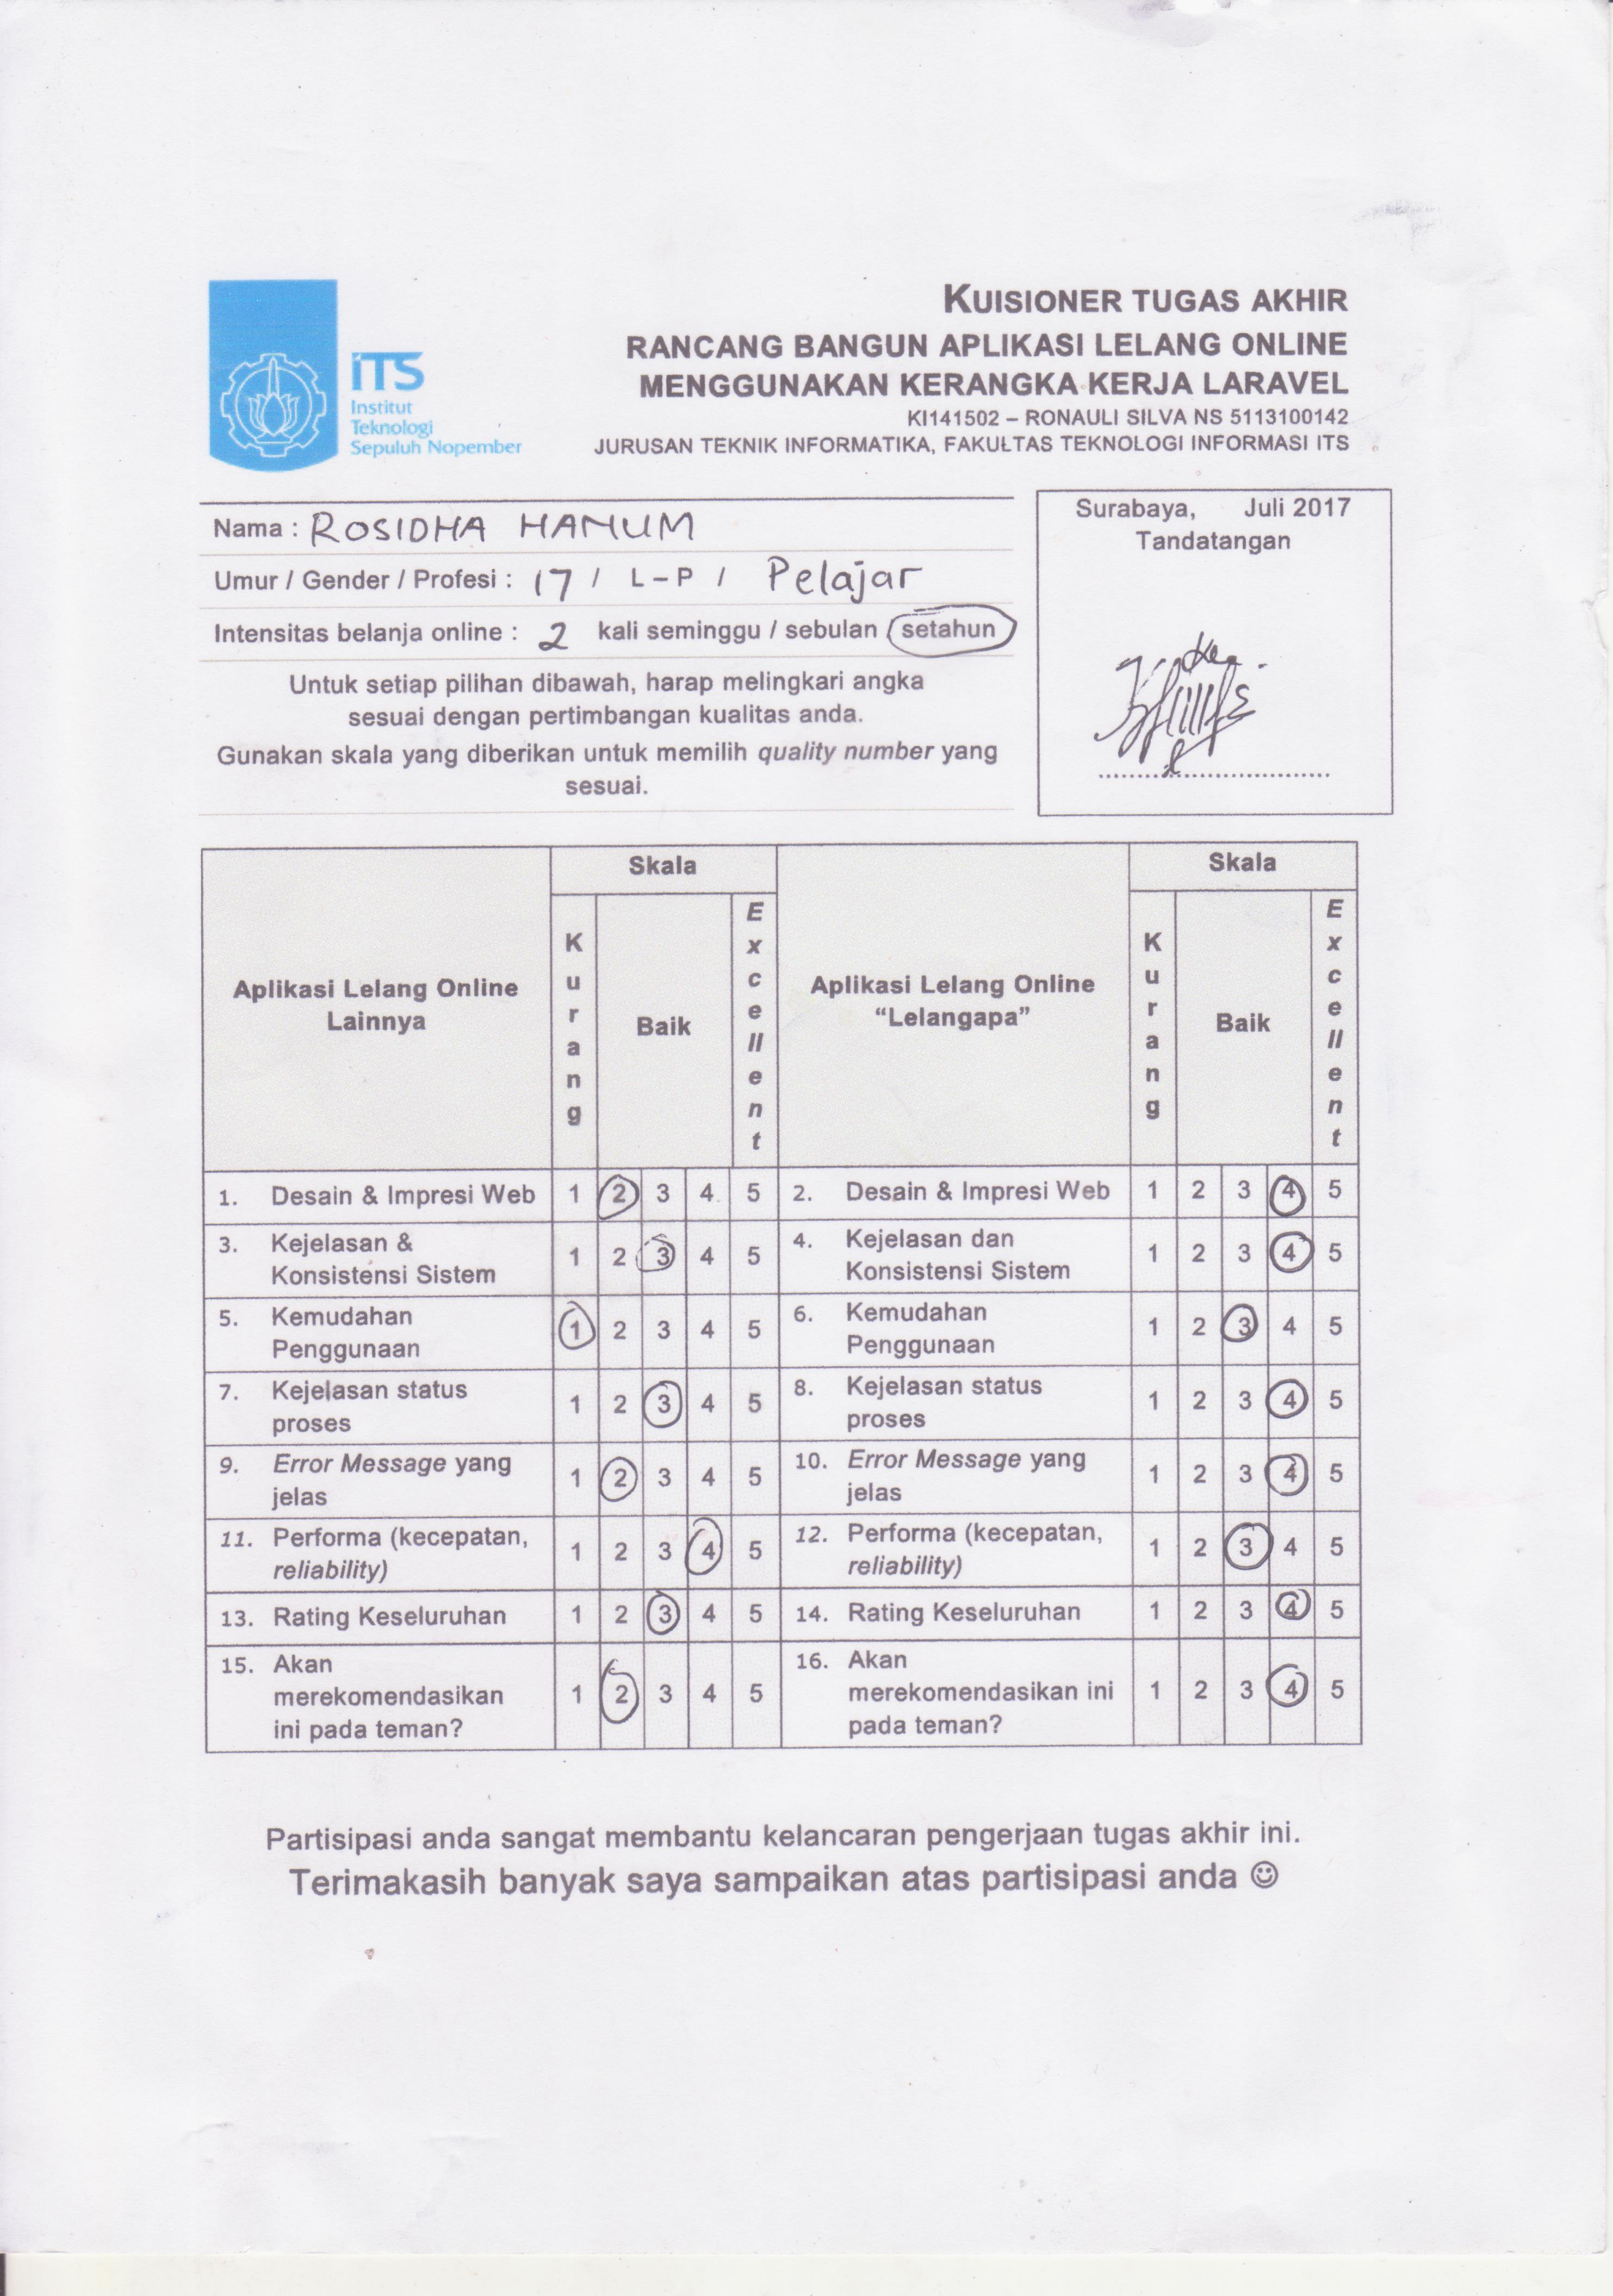
\includegraphics[width=\textwidth]{images/bab5/ujipengguna/1.jpg}
	\caption{Kuisioner Pengguna 1}
\end{figure}
\begin{figure}[H]
	\centering
	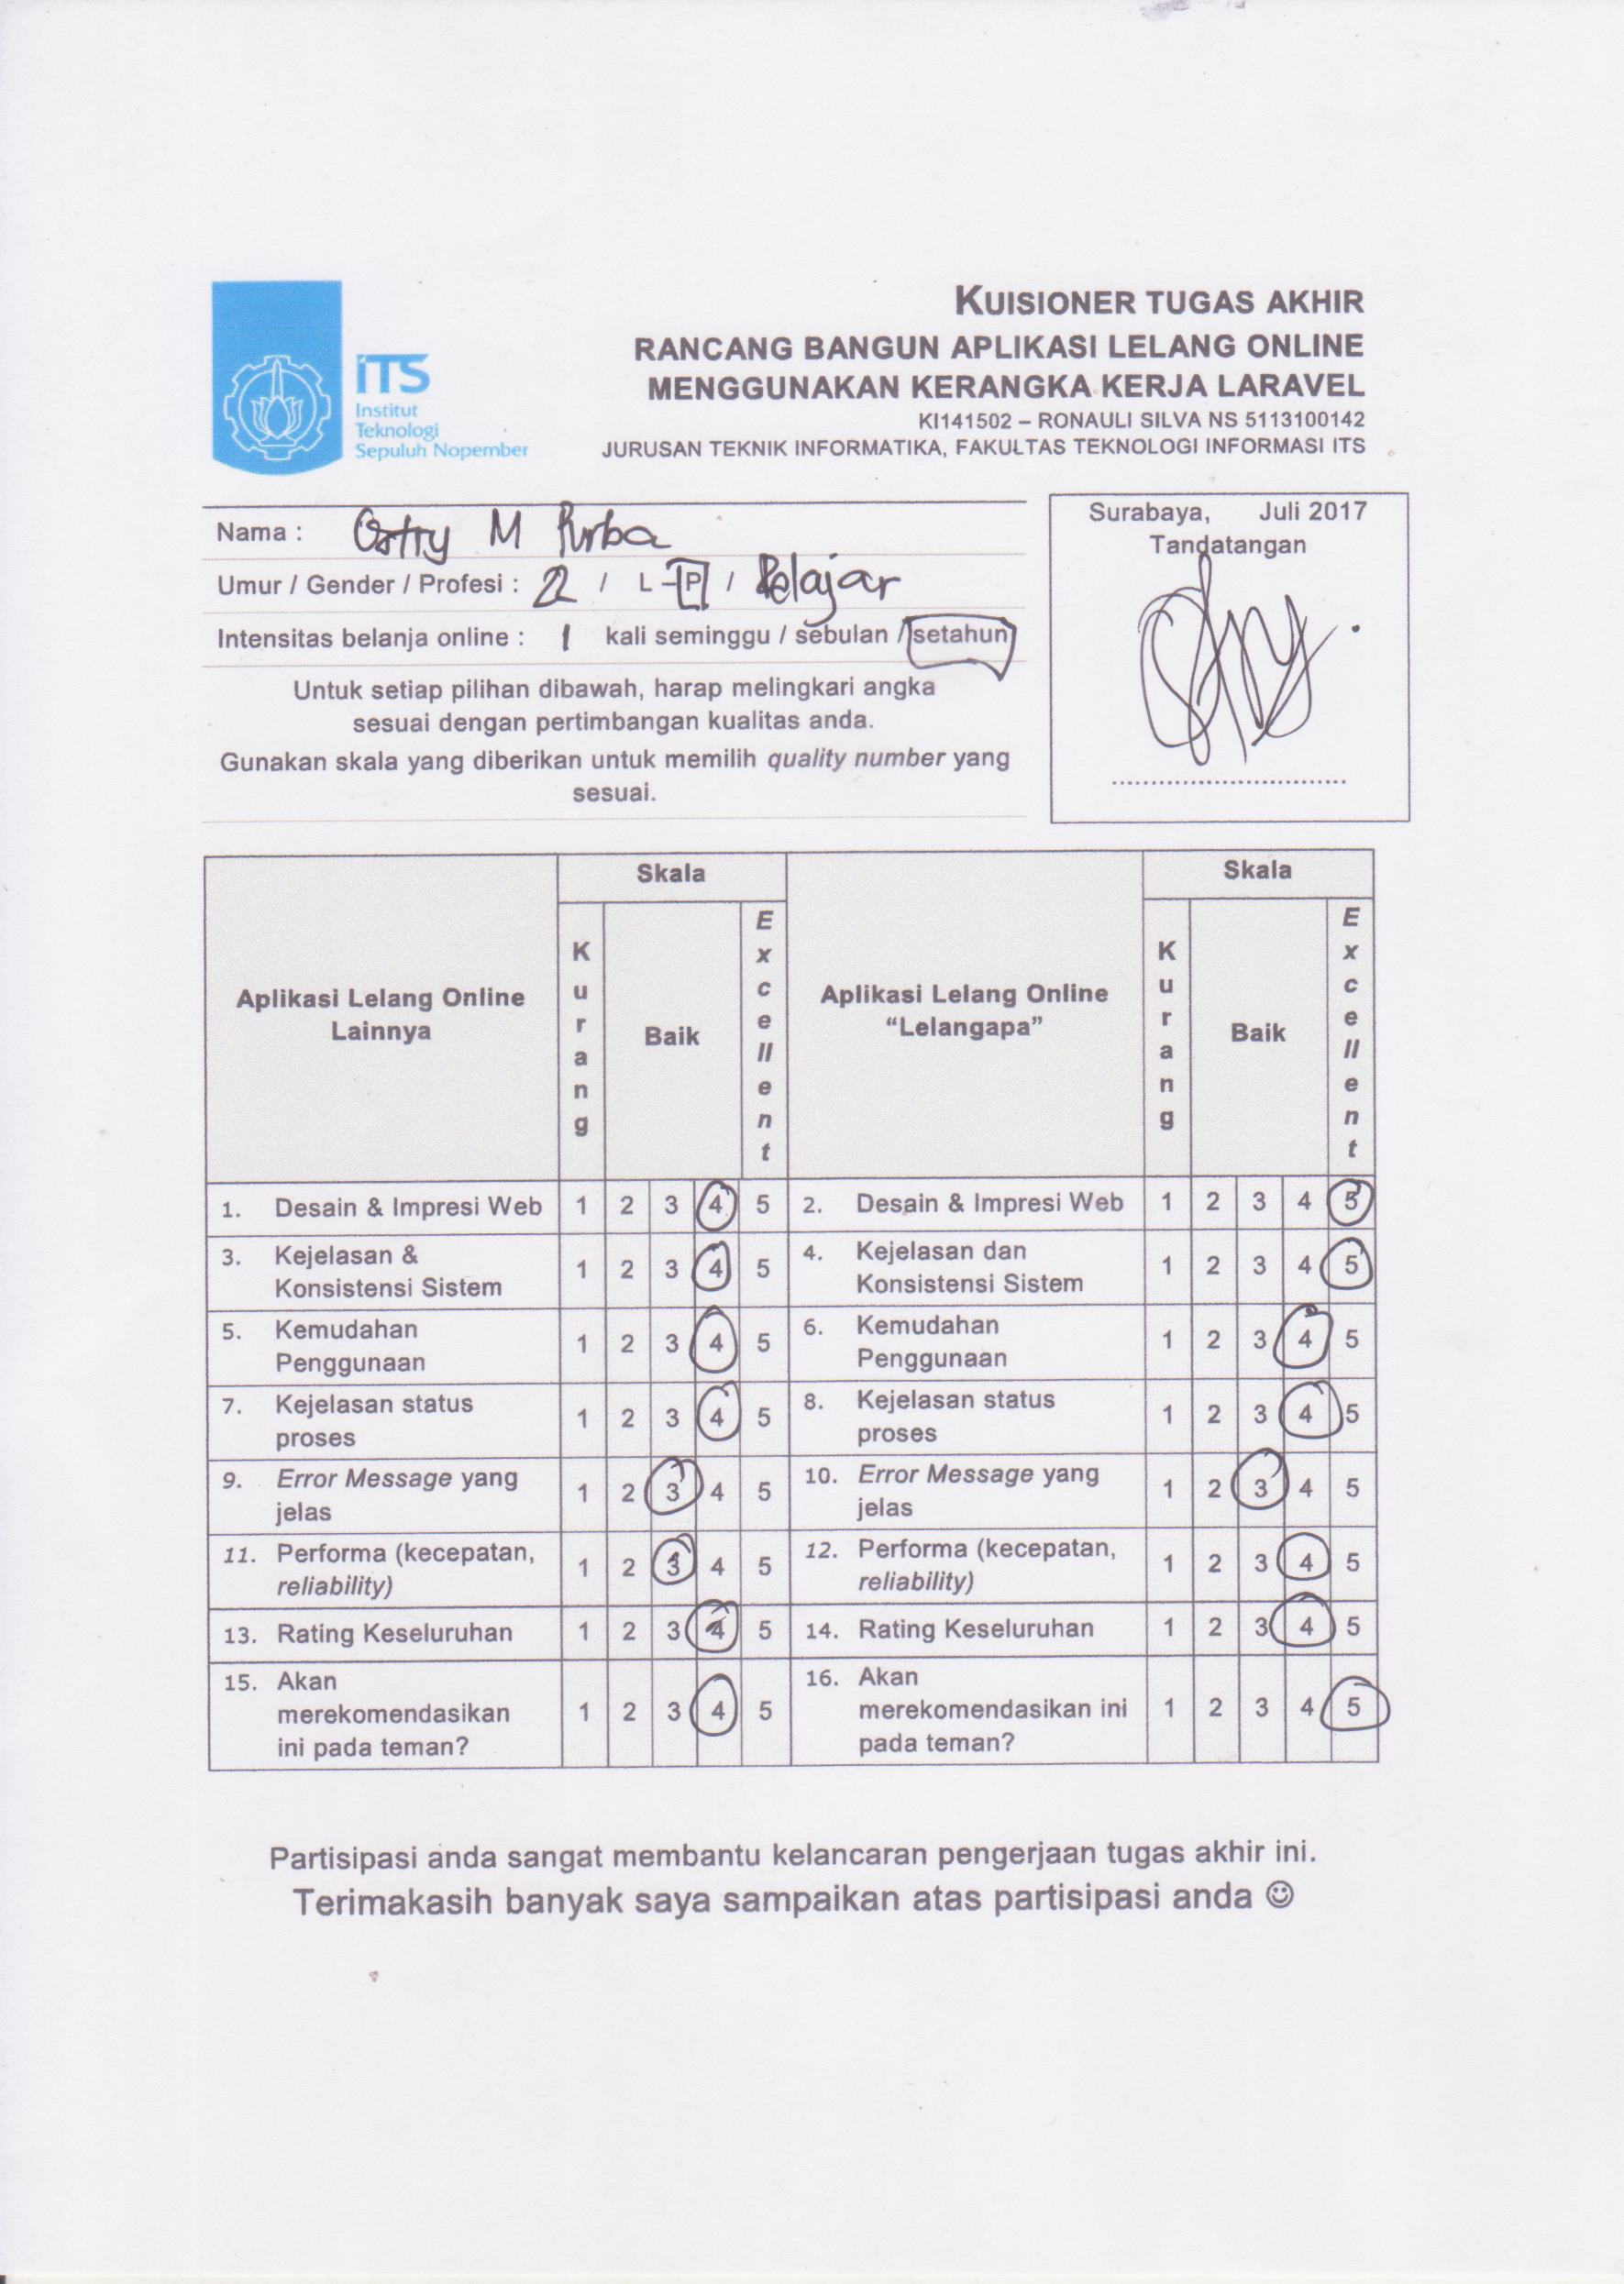
\includegraphics[width=\textwidth]{images/bab5/ujipengguna/2.jpg}
	\caption{Kuisioner Pengguna 2}
\end{figure}
\begin{figure}[H]
	\centering
	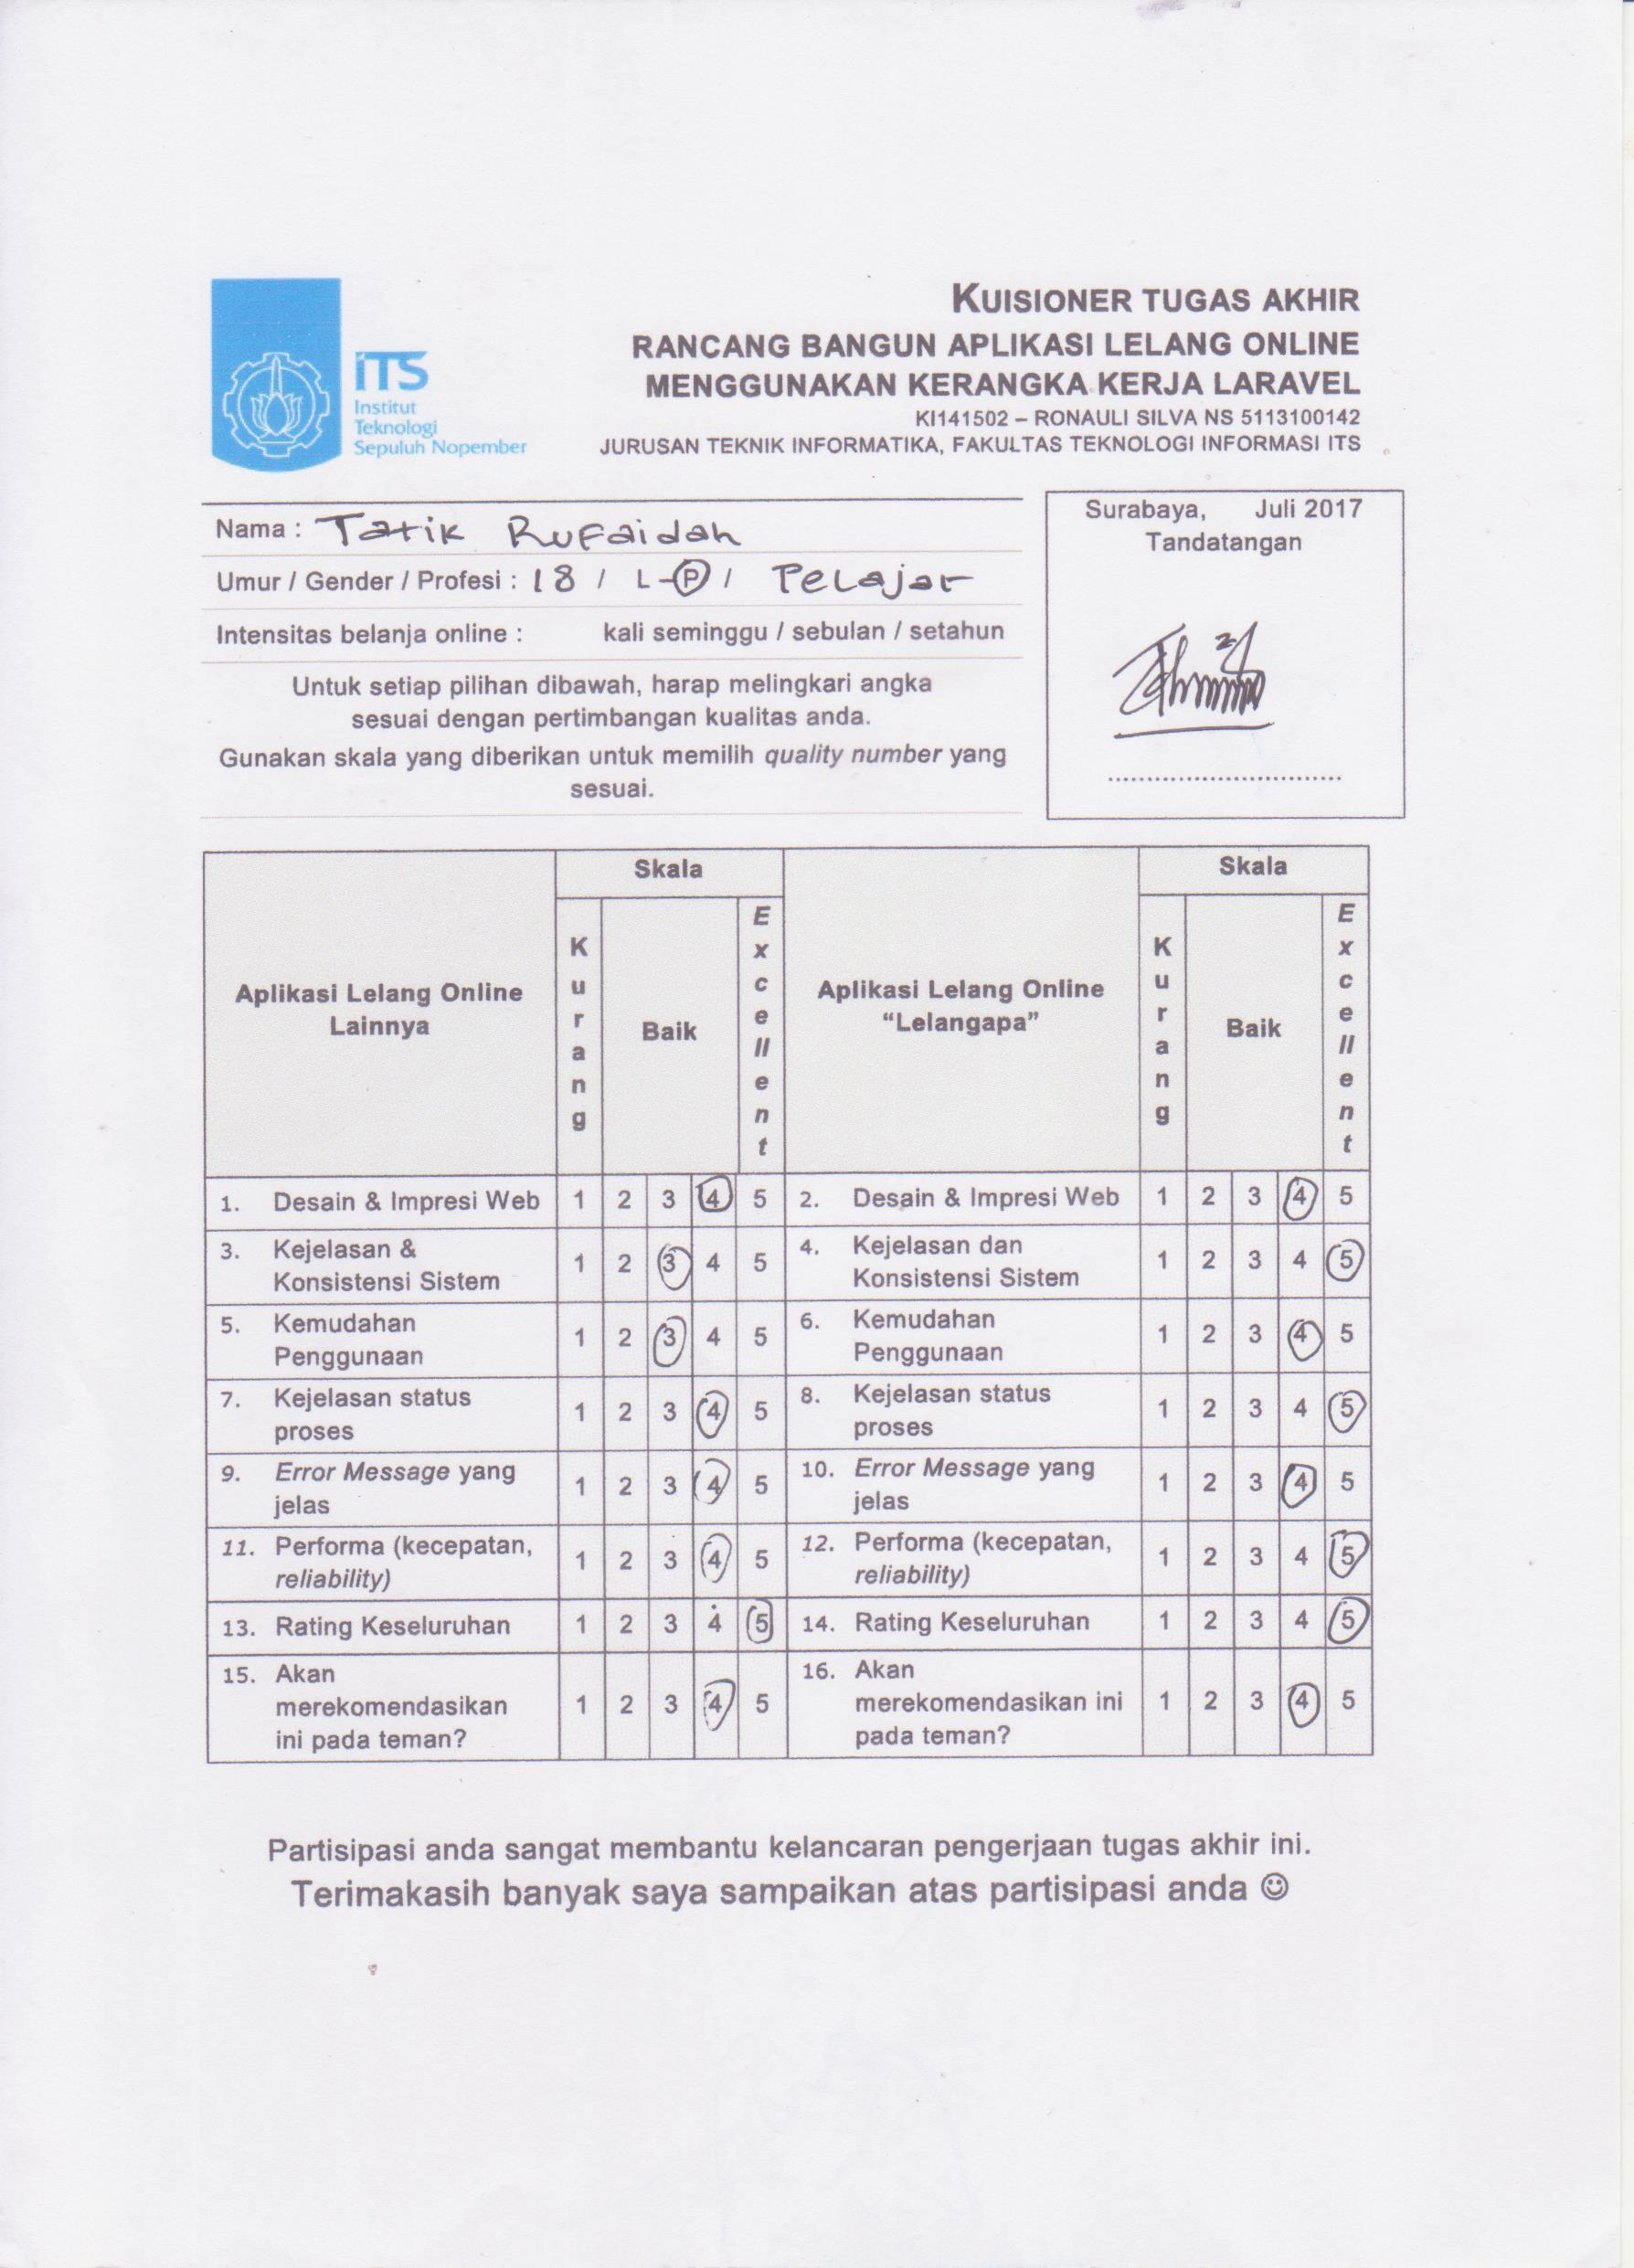
\includegraphics[width=\textwidth]{images/bab5/ujipengguna/3.jpg}
	\caption{Kuisioner Pengguna 3}
\end{figure}
\begin{figure}[H]
	\centering
	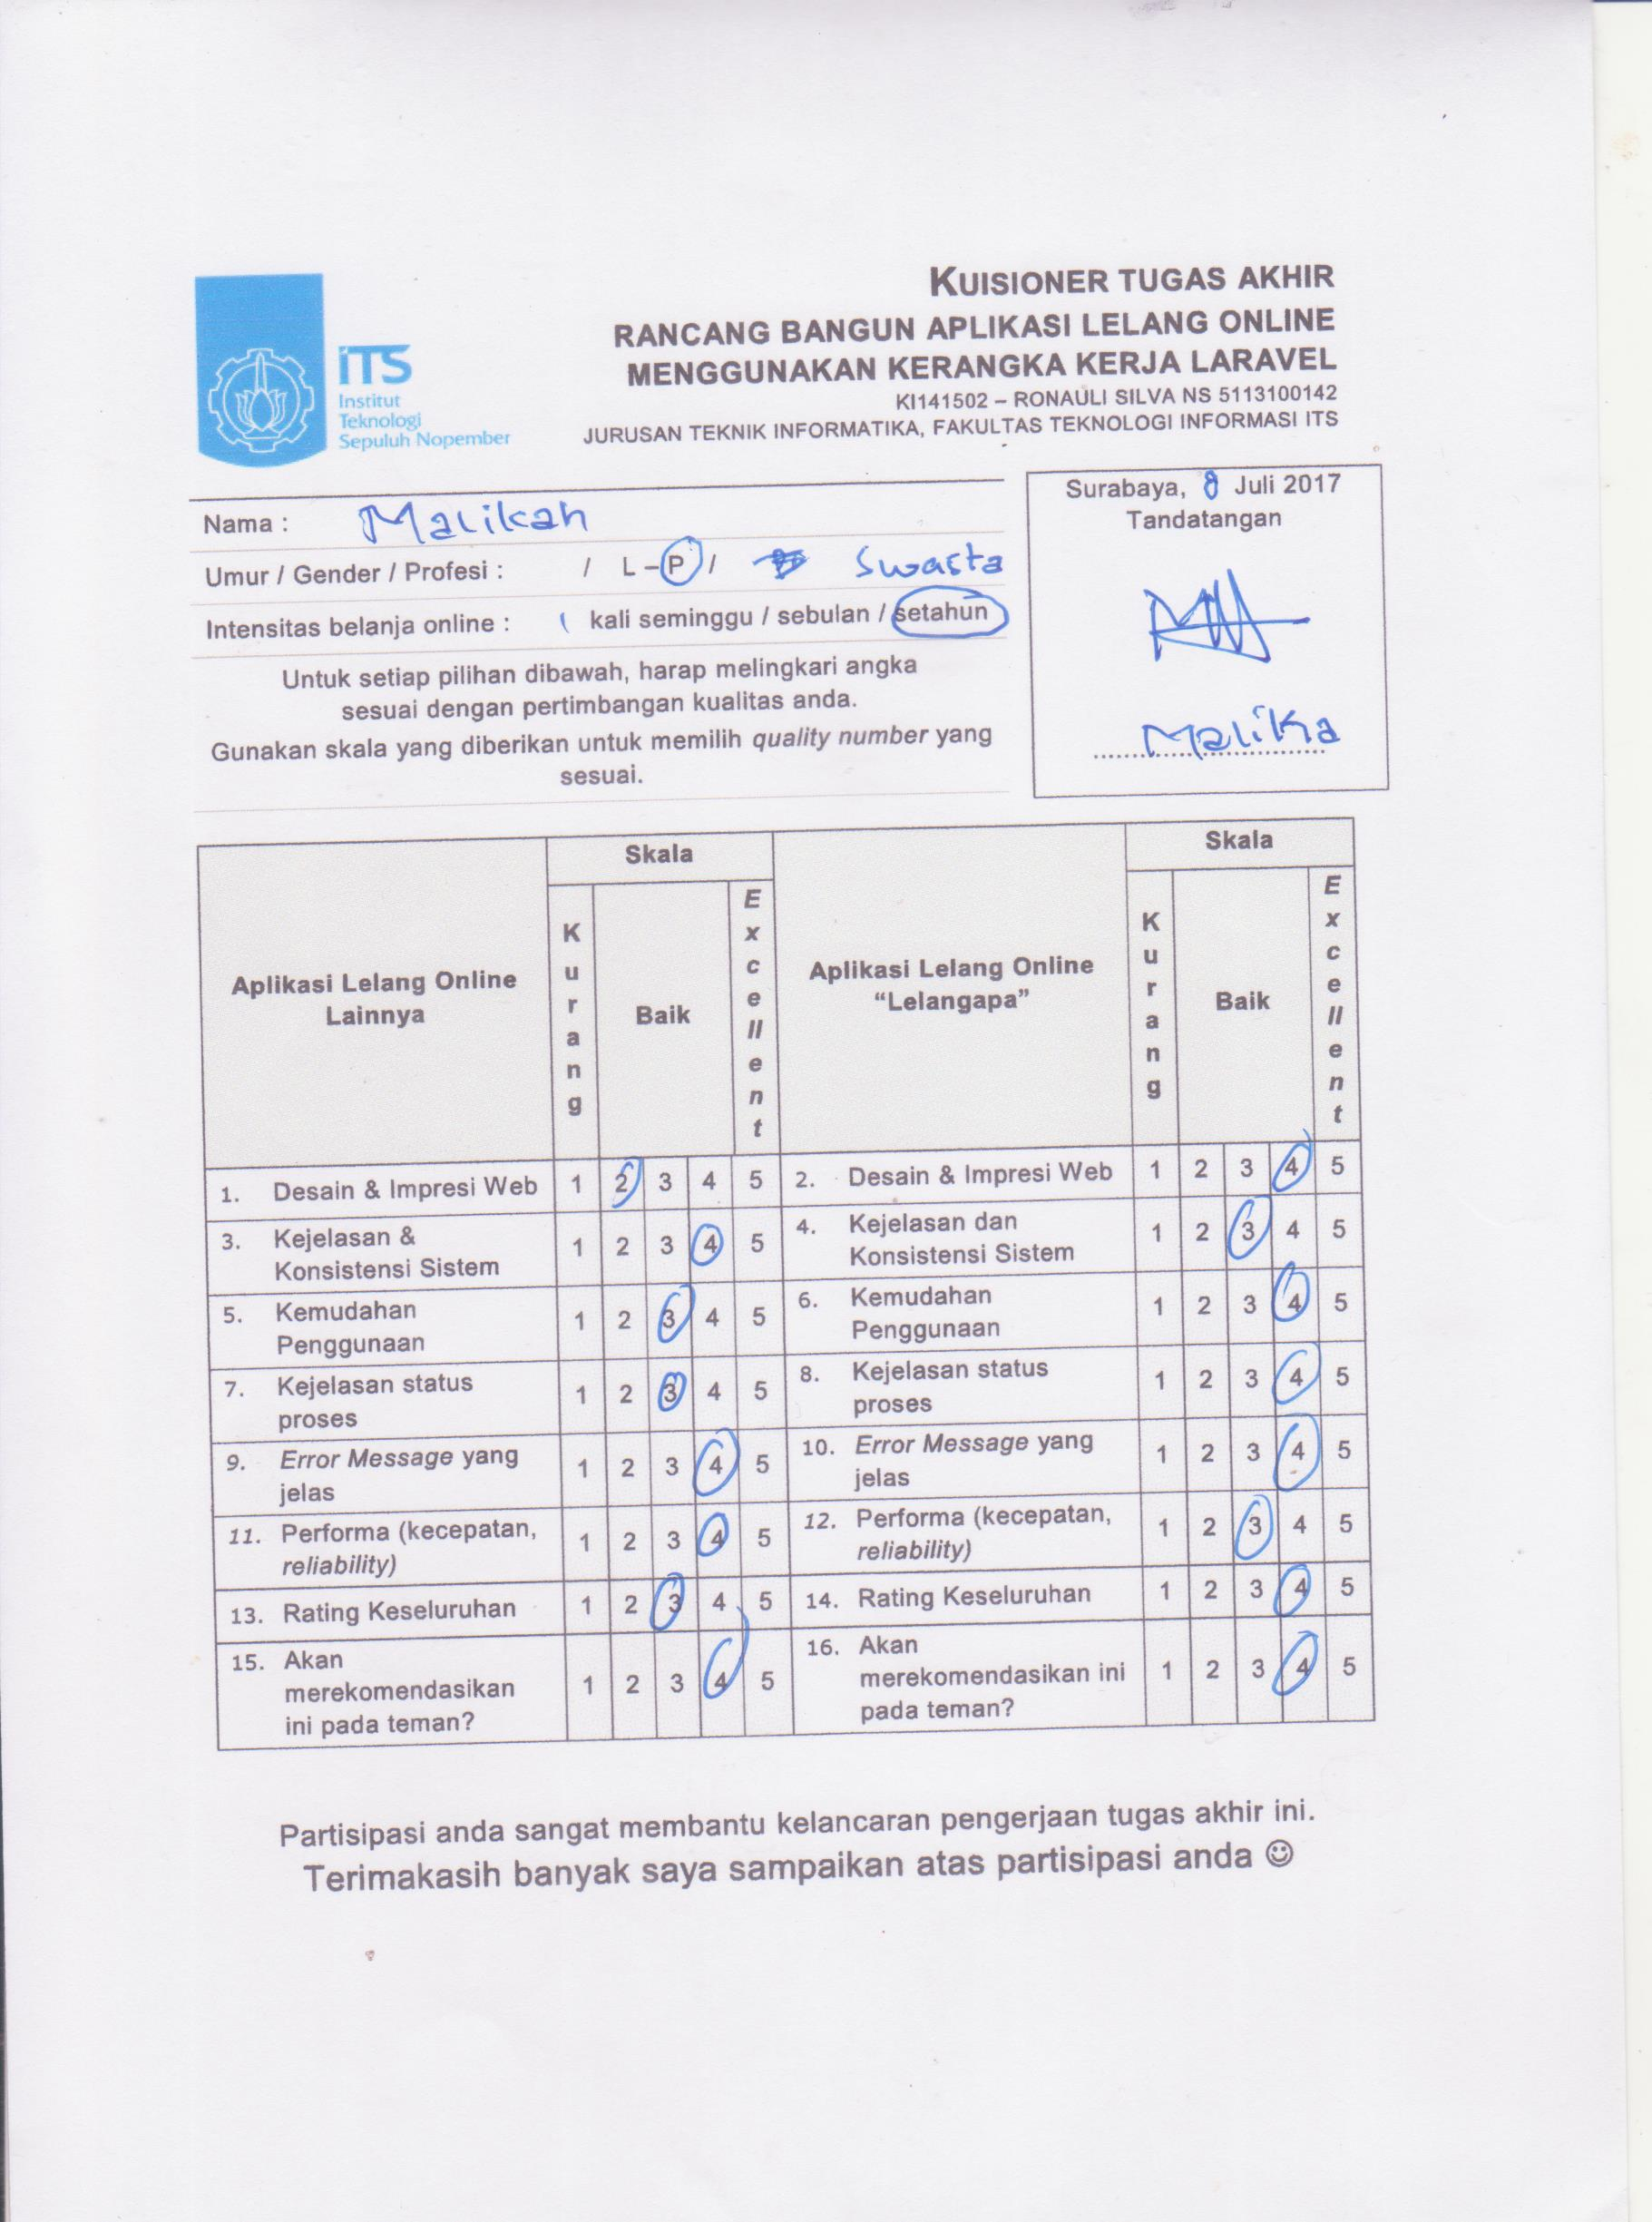
\includegraphics[width=\textwidth]{images/bab5/ujipengguna/4.jpg}
	\caption{Kuisioner Pengguna 4}
\end{figure}
\begin{figure}[H]
	\centering
	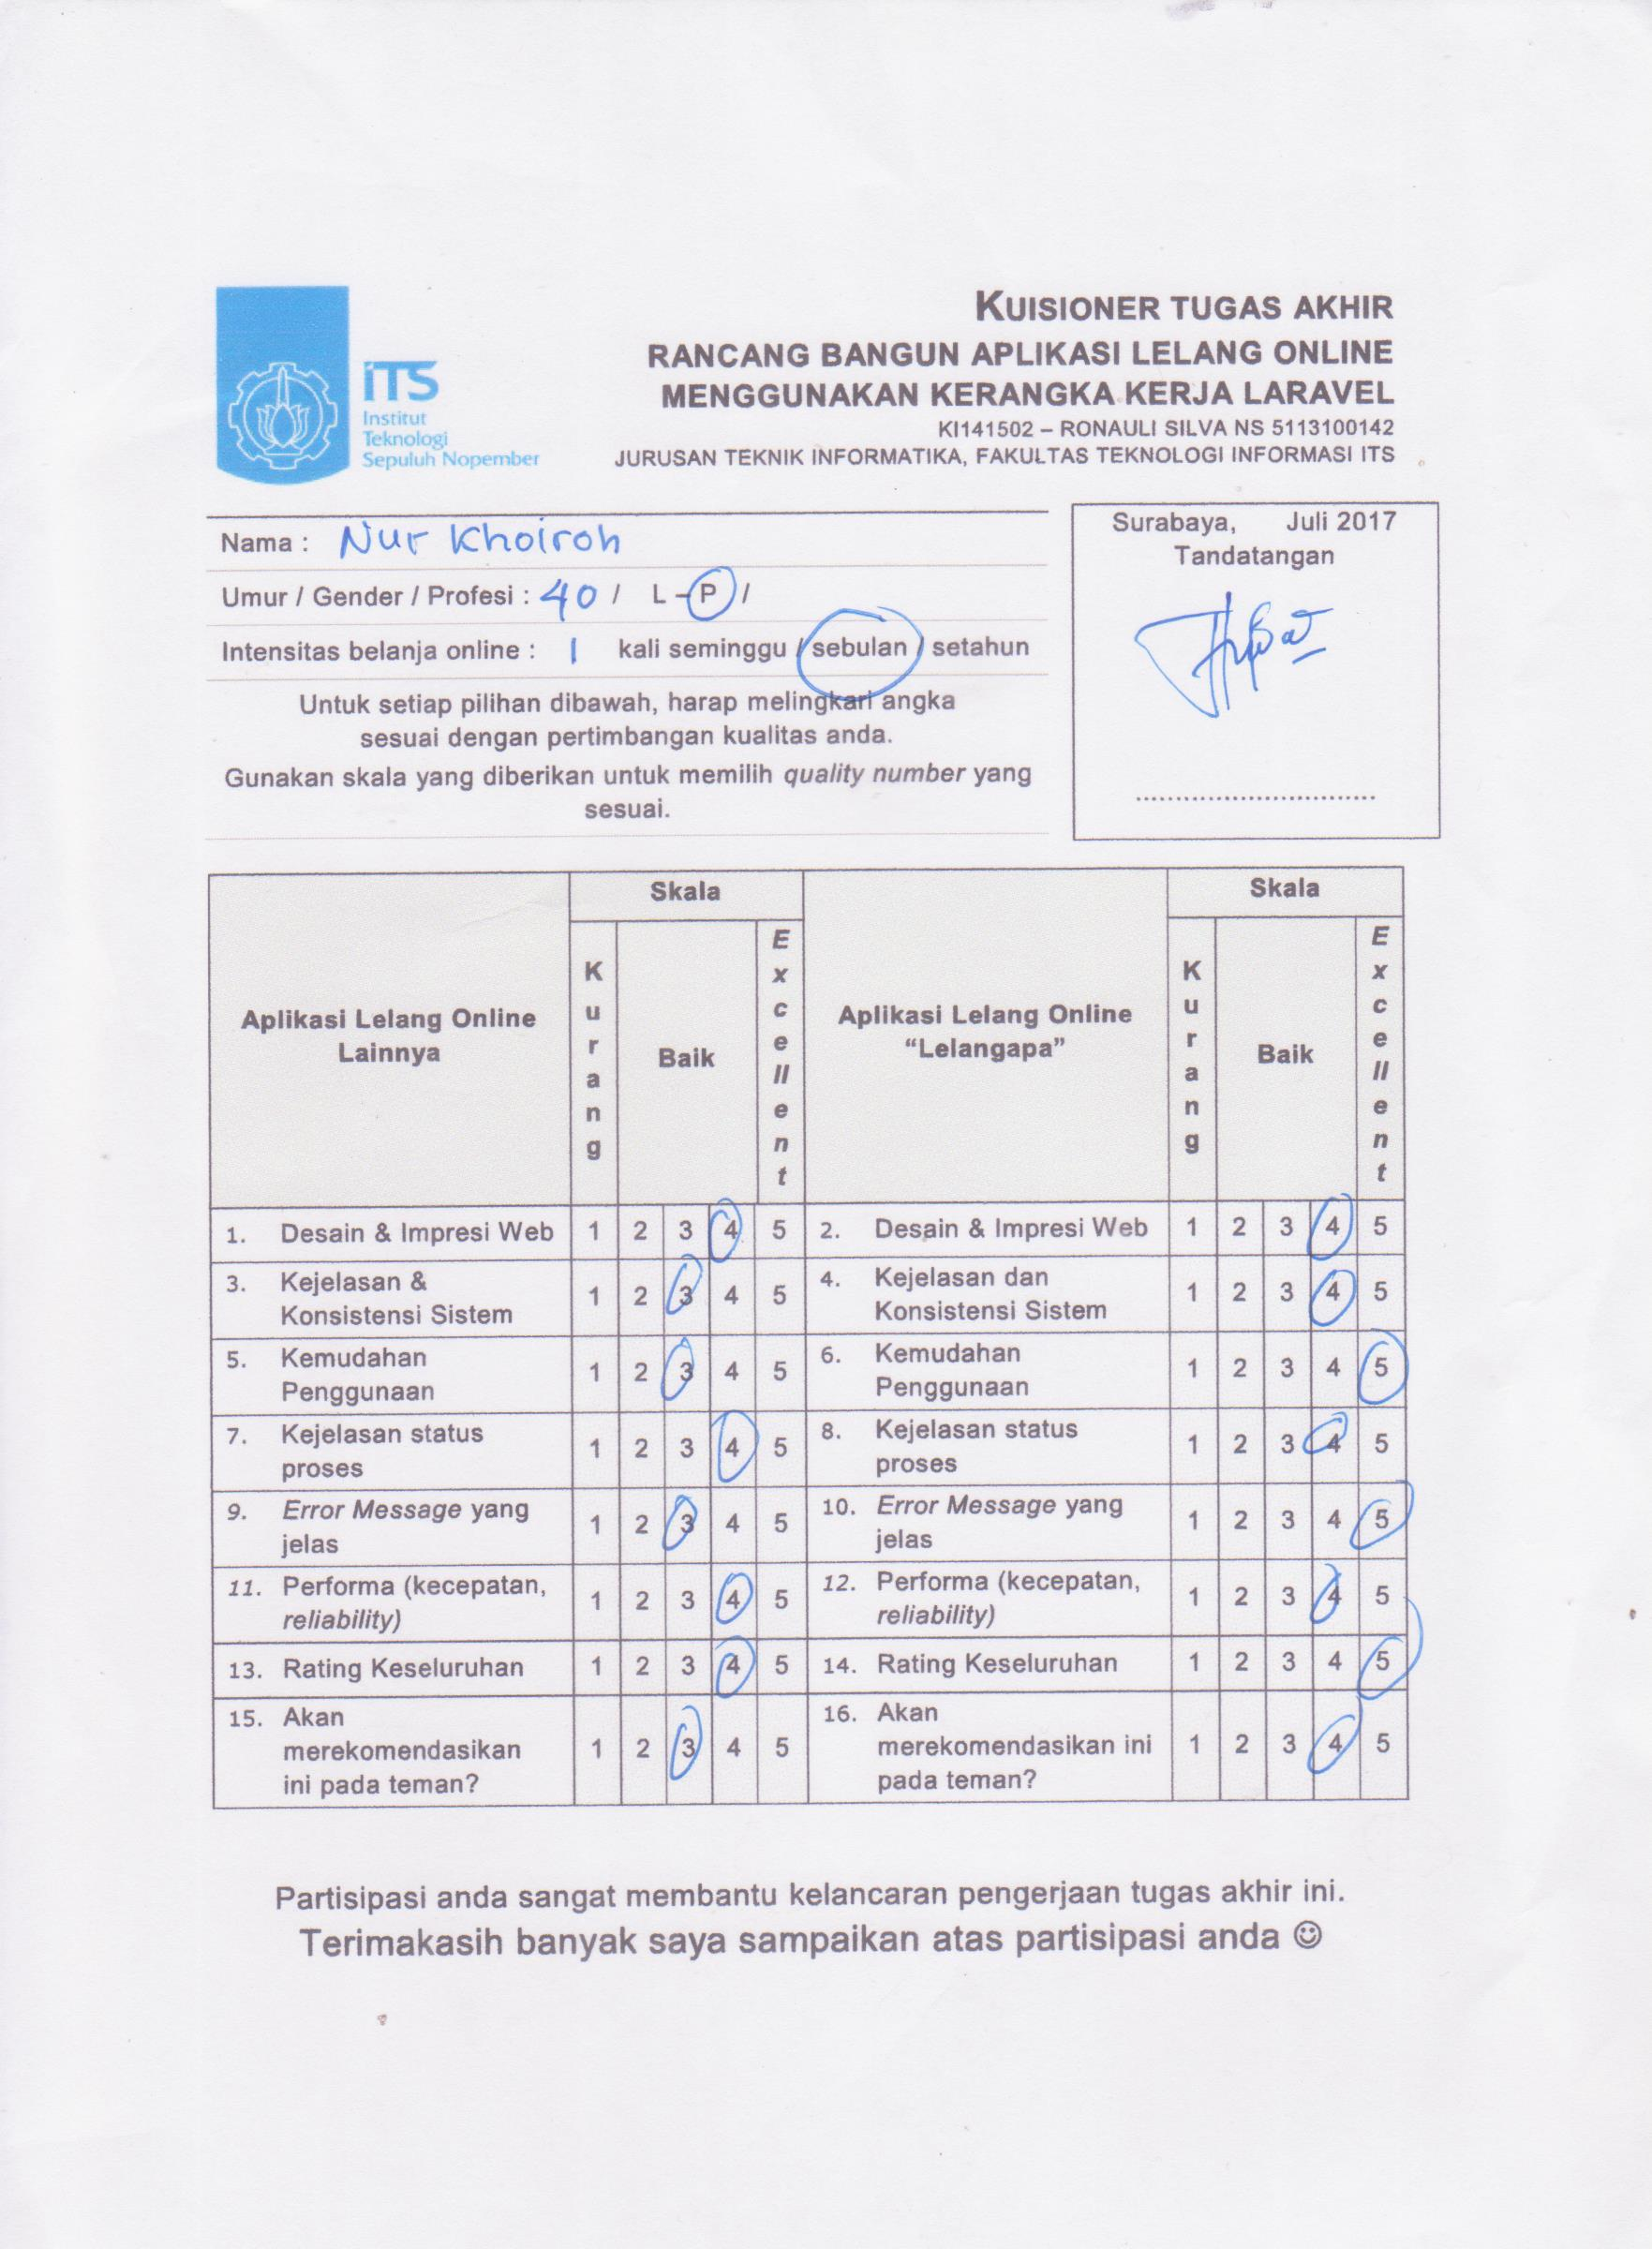
\includegraphics[width=\textwidth]{images/bab5/ujipengguna/5.jpg}
	\caption{Kuisioner Pengguna 5}
\end{figure}
\begin{figure}[H]
	\centering
	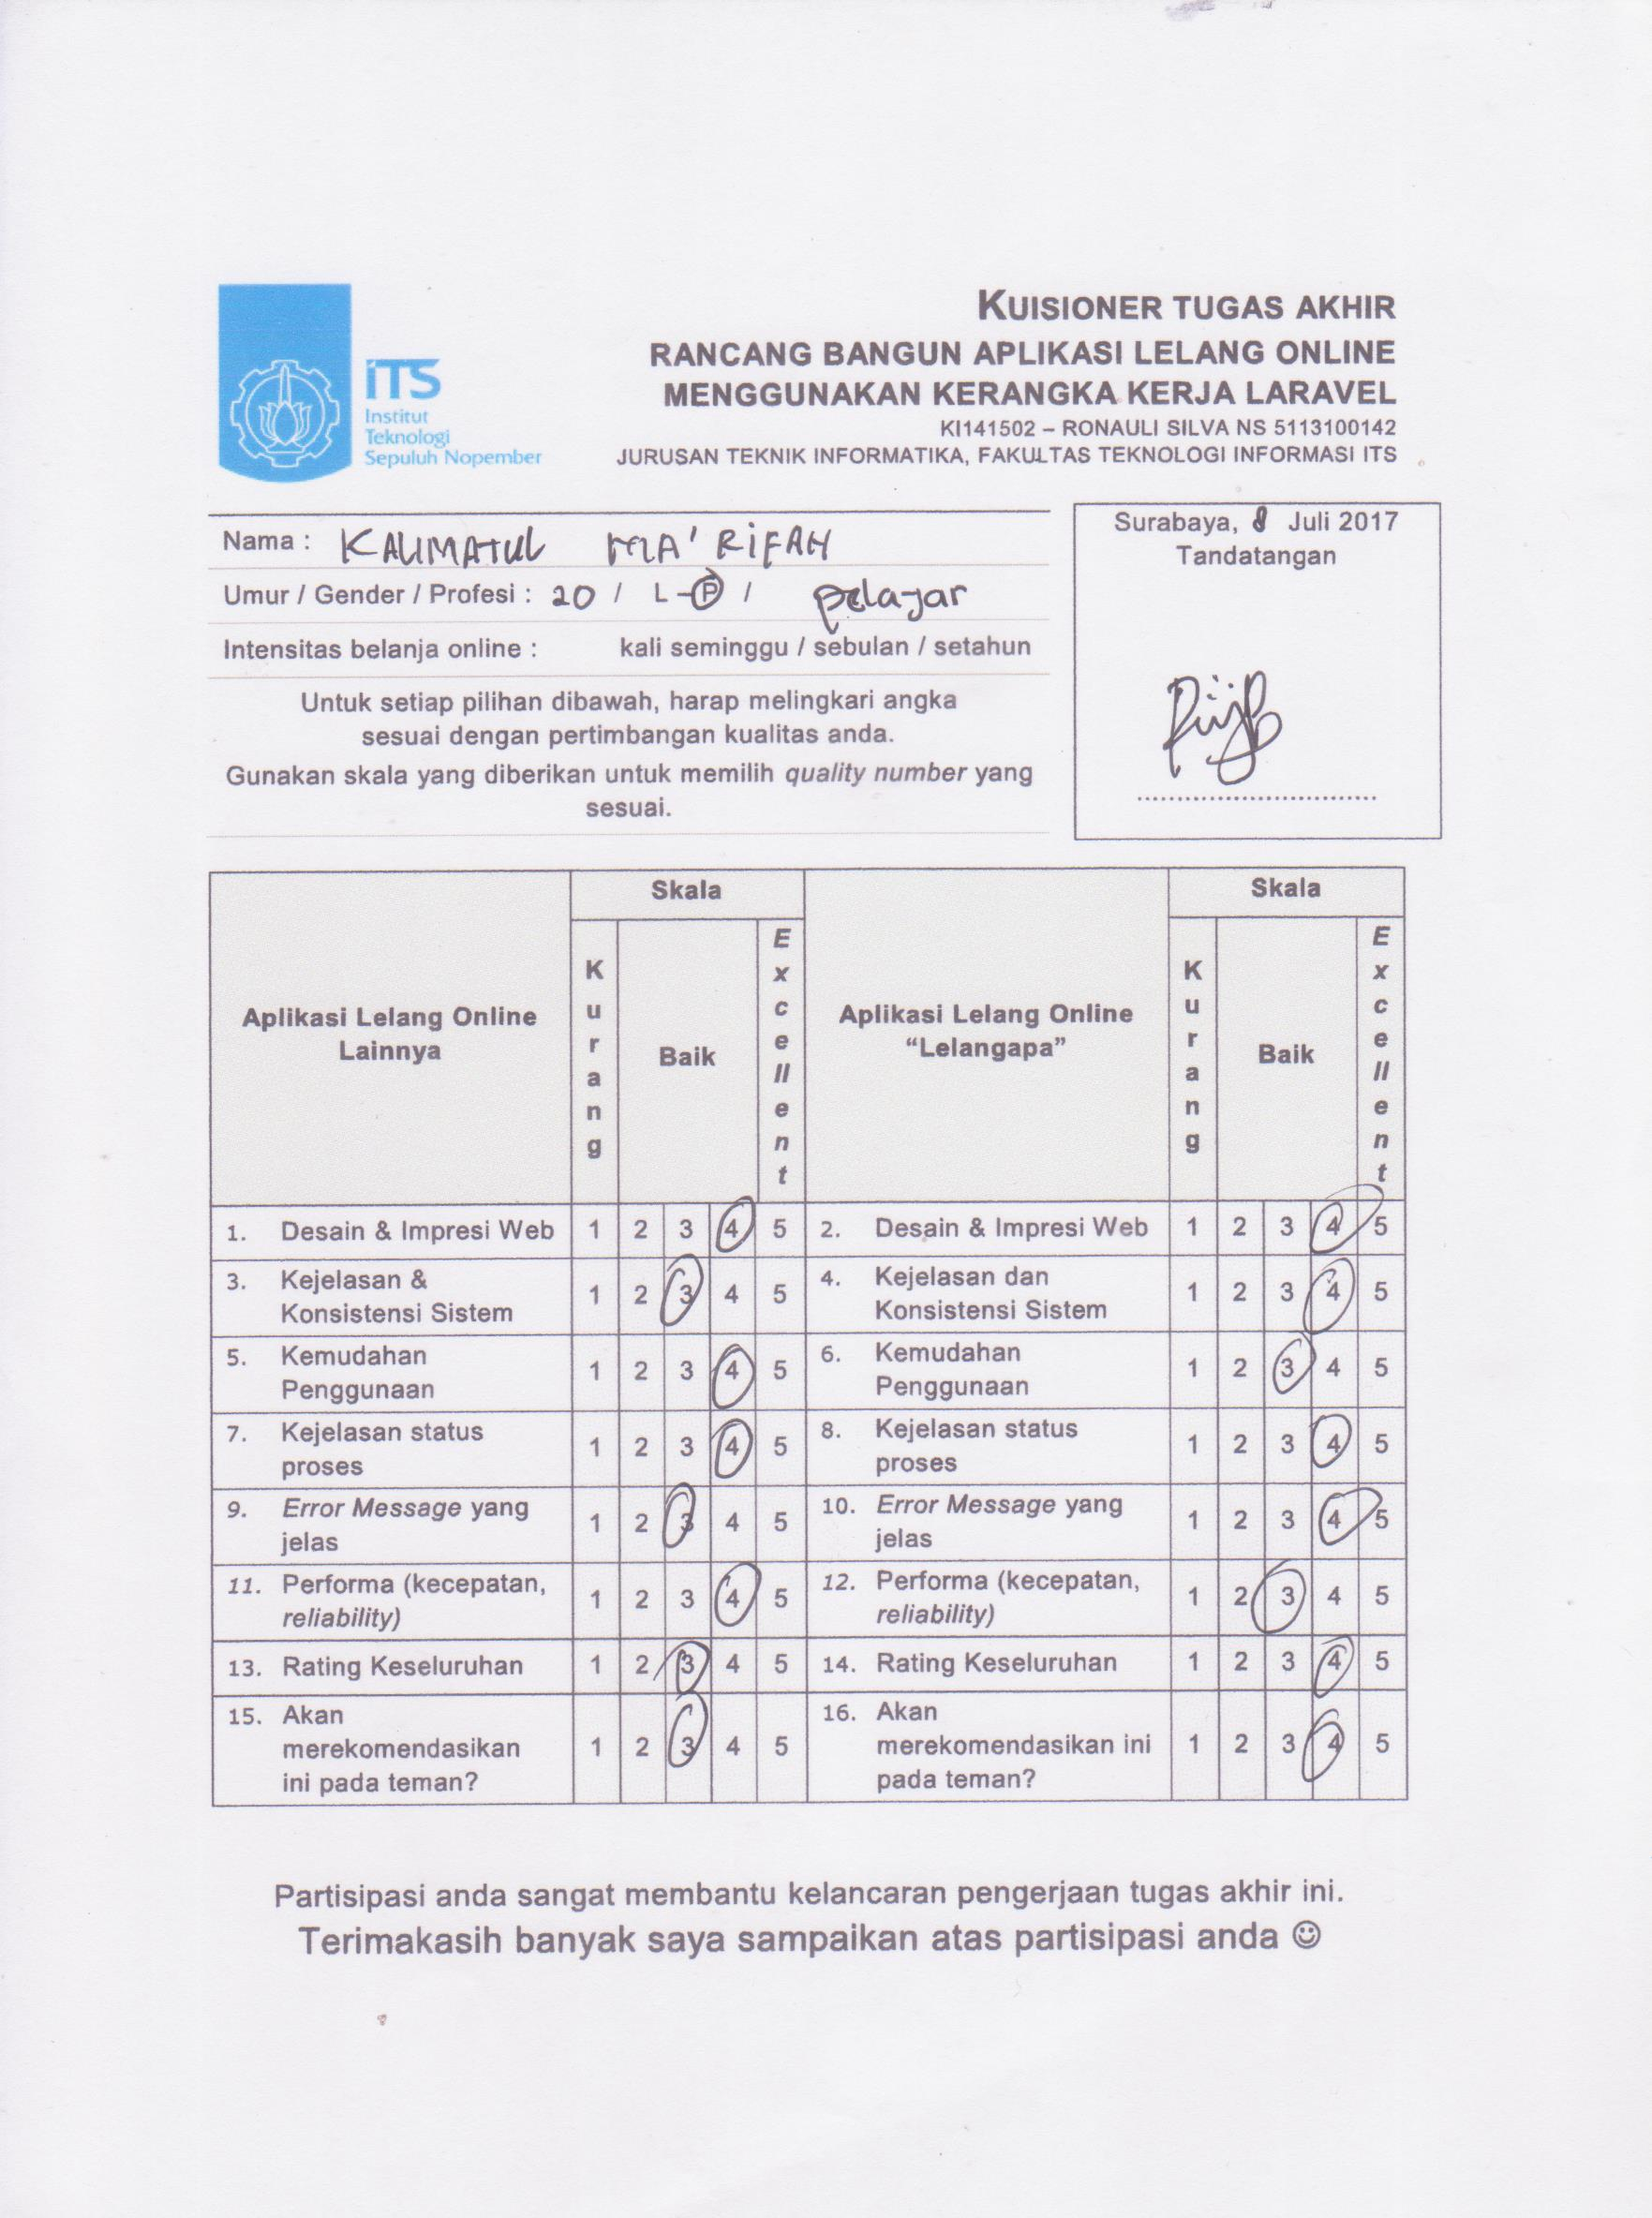
\includegraphics[width=\textwidth]{images/bab5/ujipengguna/6.jpg}
	\caption{Kuisioner Pengguna 6}
\end{figure}
\begin{figure}[H]
	\centering
	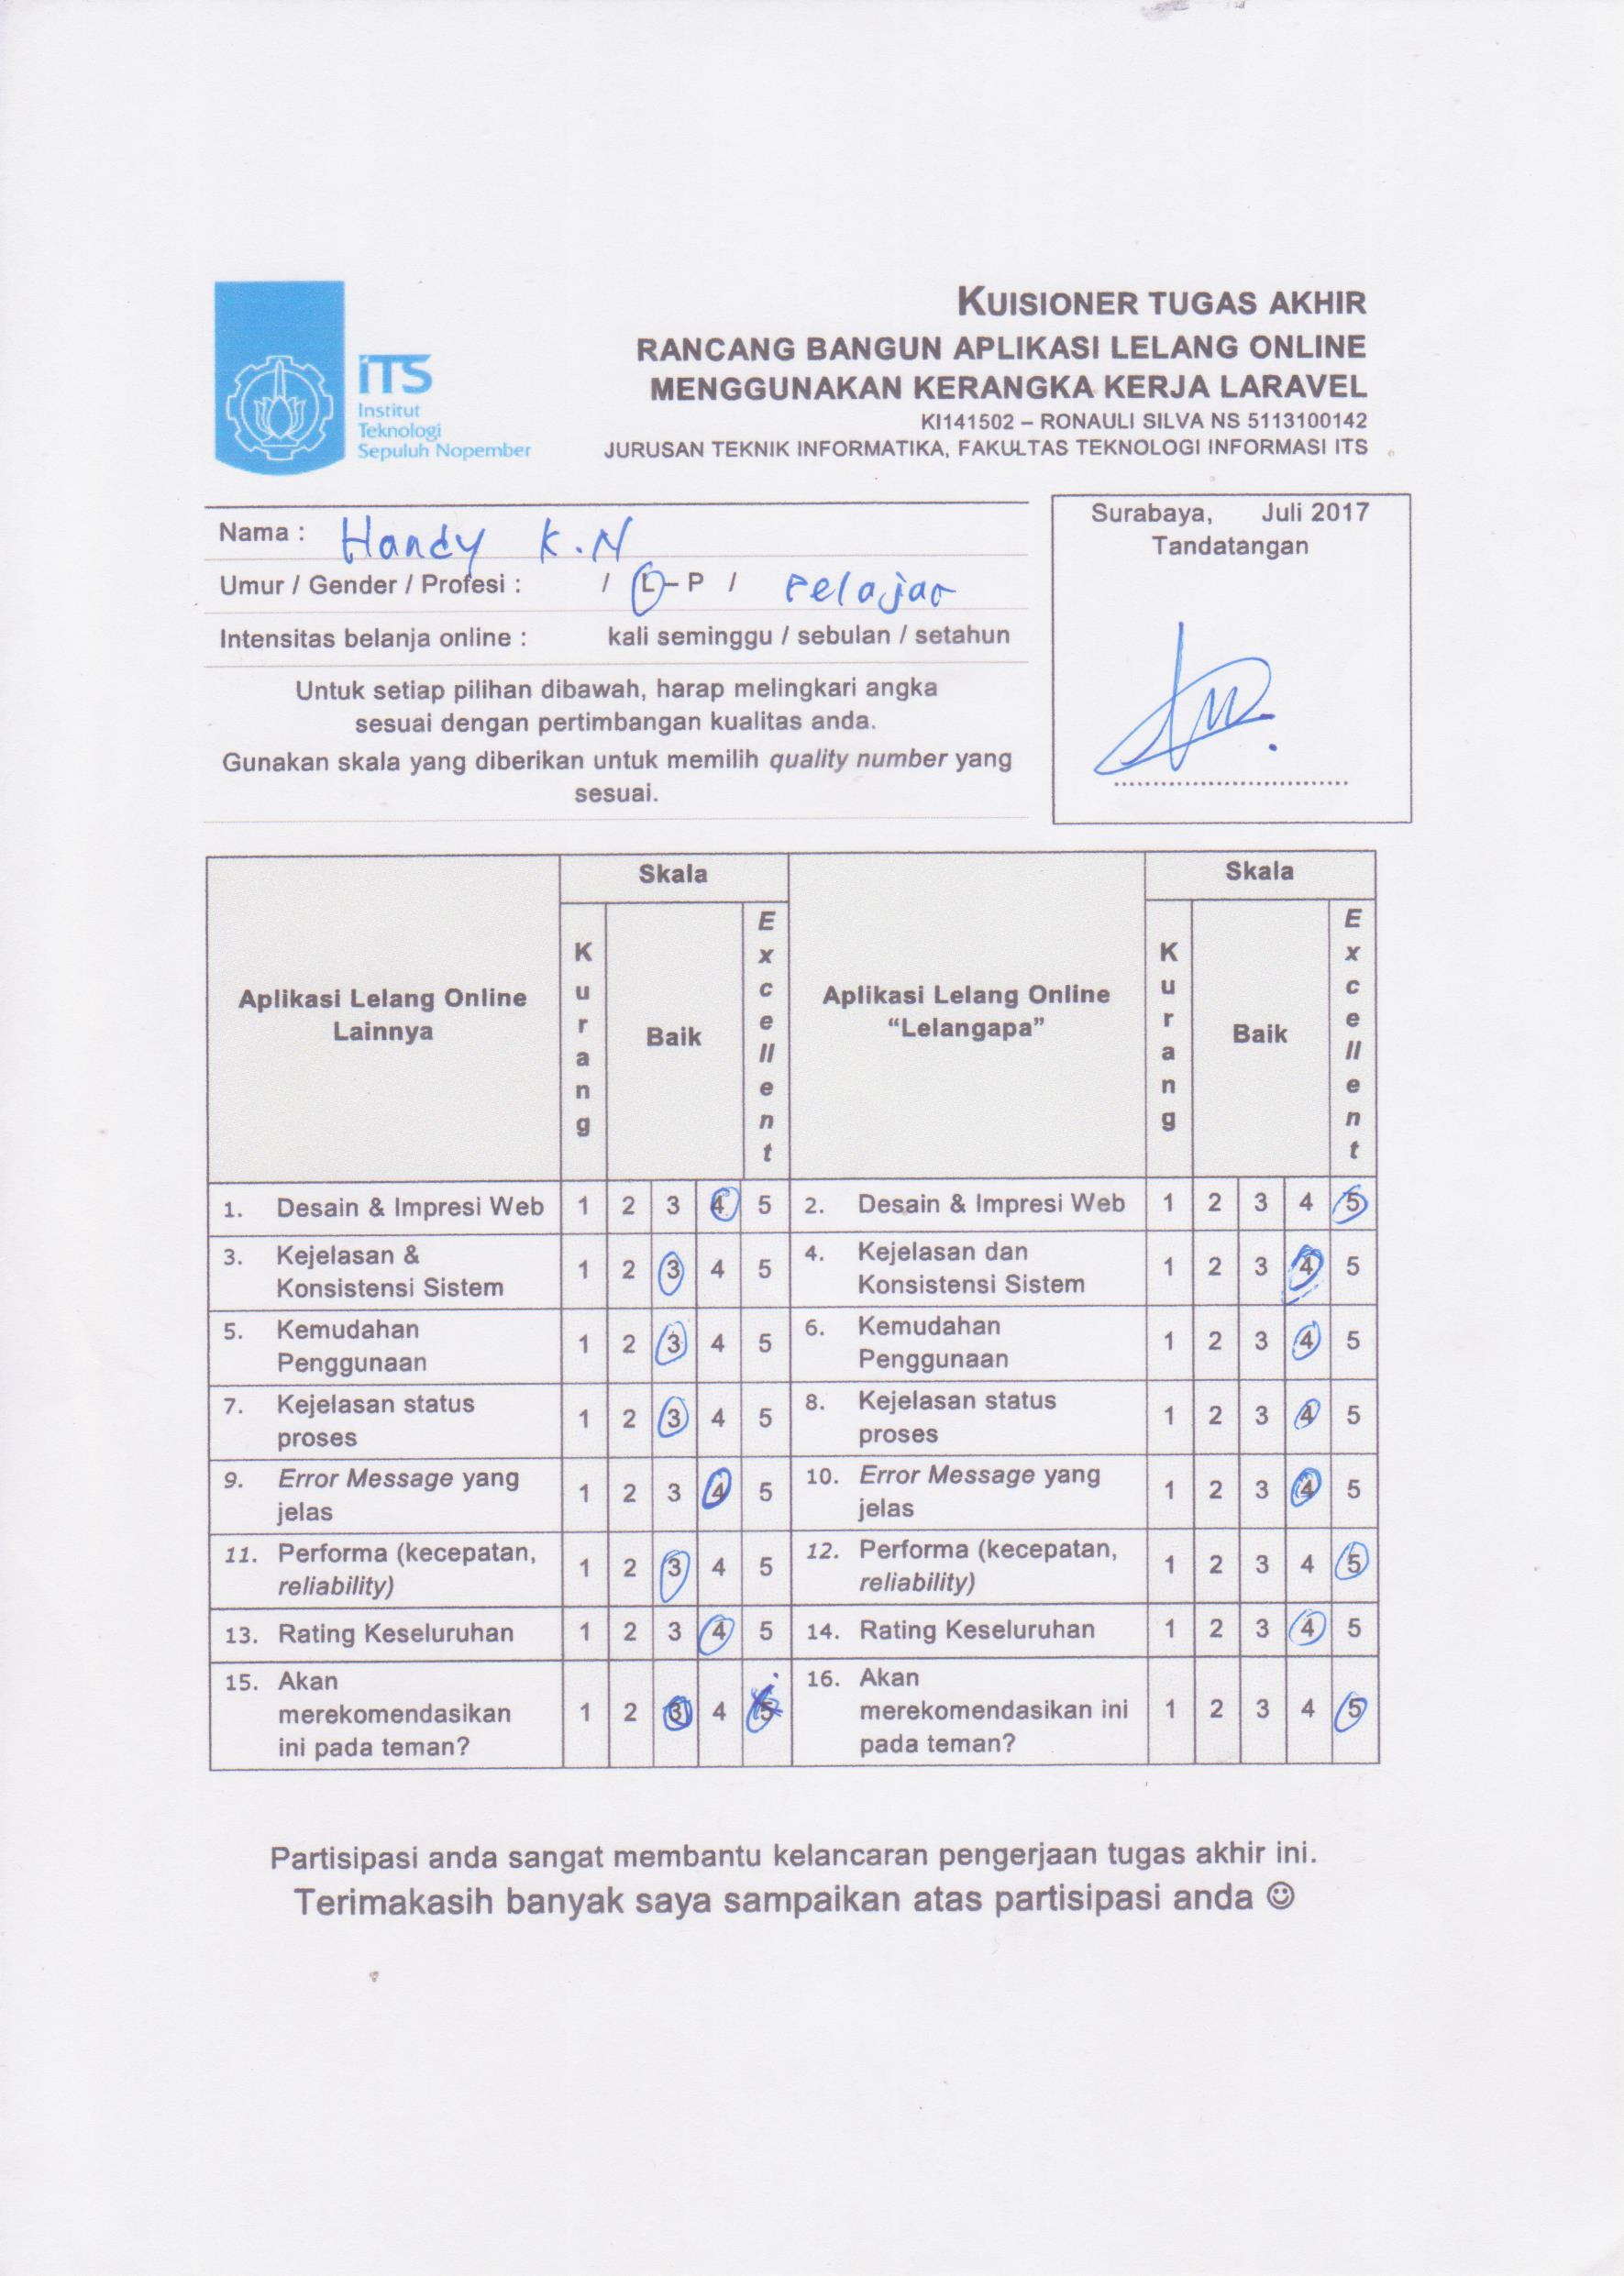
\includegraphics[width=\textwidth]{images/bab5/ujipengguna/7.jpg}
	\caption{Kuisioner Pengguna 7}
\end{figure}
\begin{figure}[H]
	\centering
	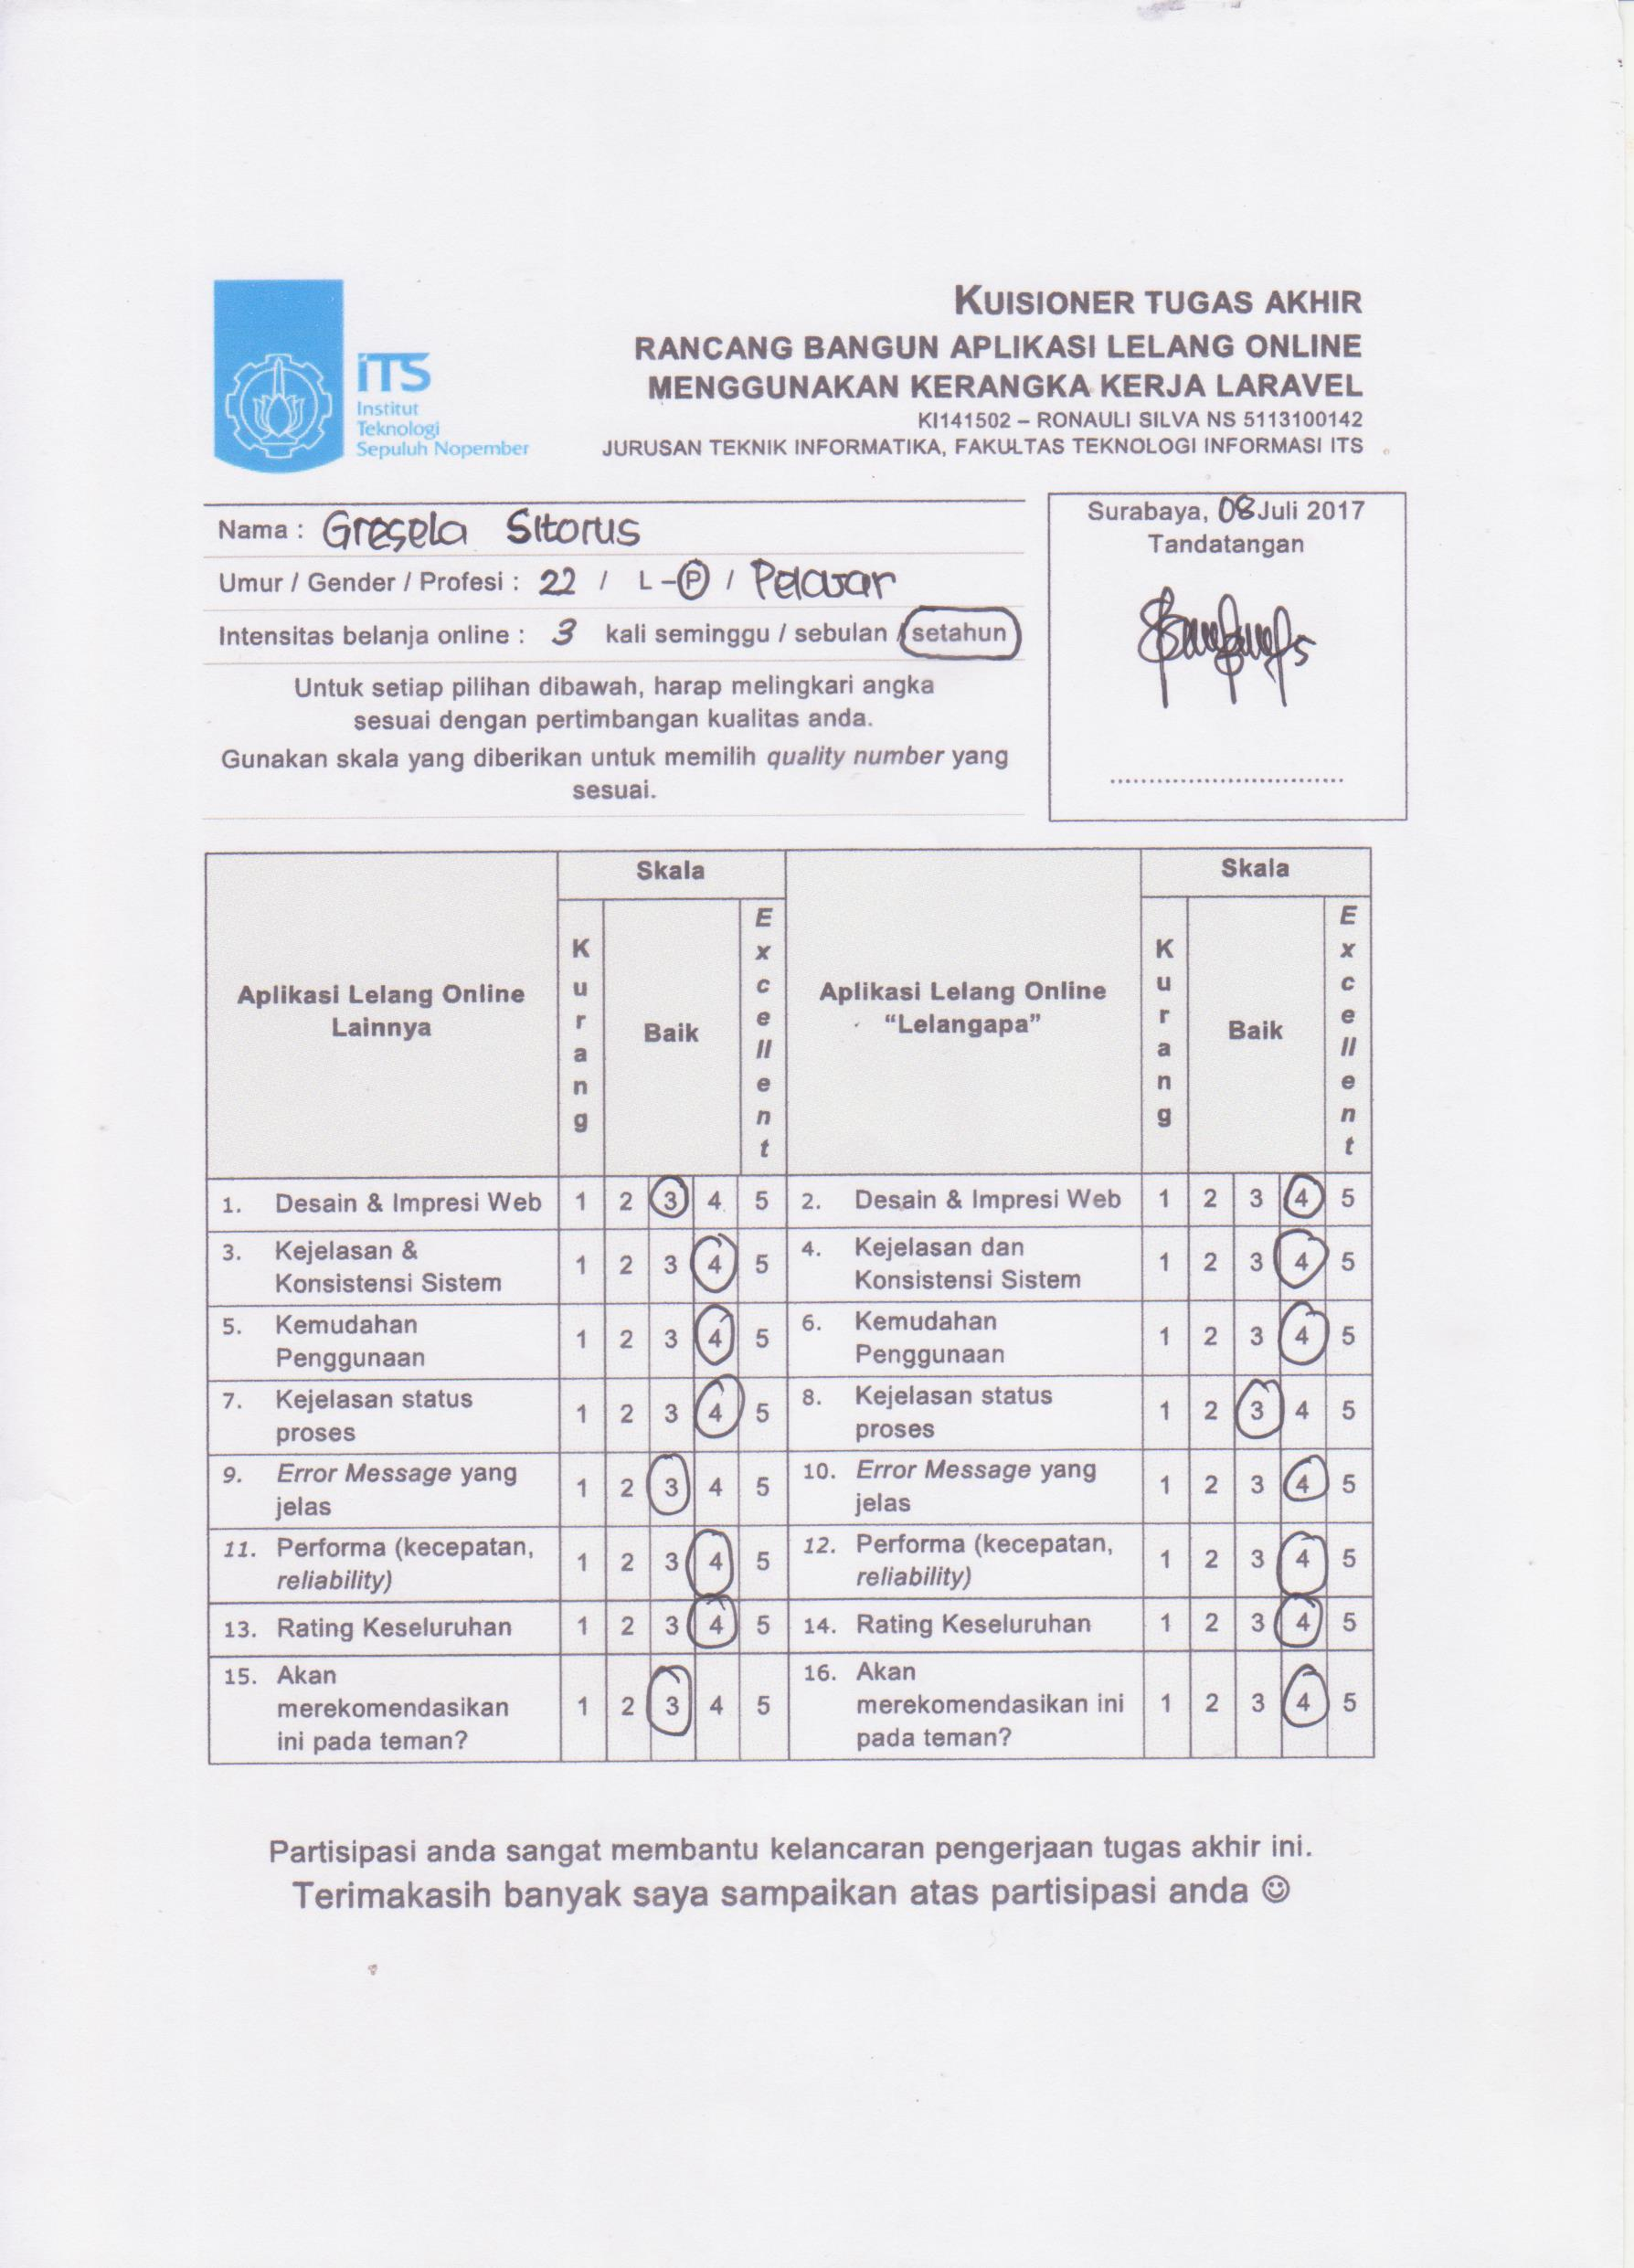
\includegraphics[width=\textwidth]{images/bab5/ujipengguna/8.jpg}
	\caption{Kuisioner Pengguna 8}
\end{figure}
\begin{figure}[H]
	\centering
	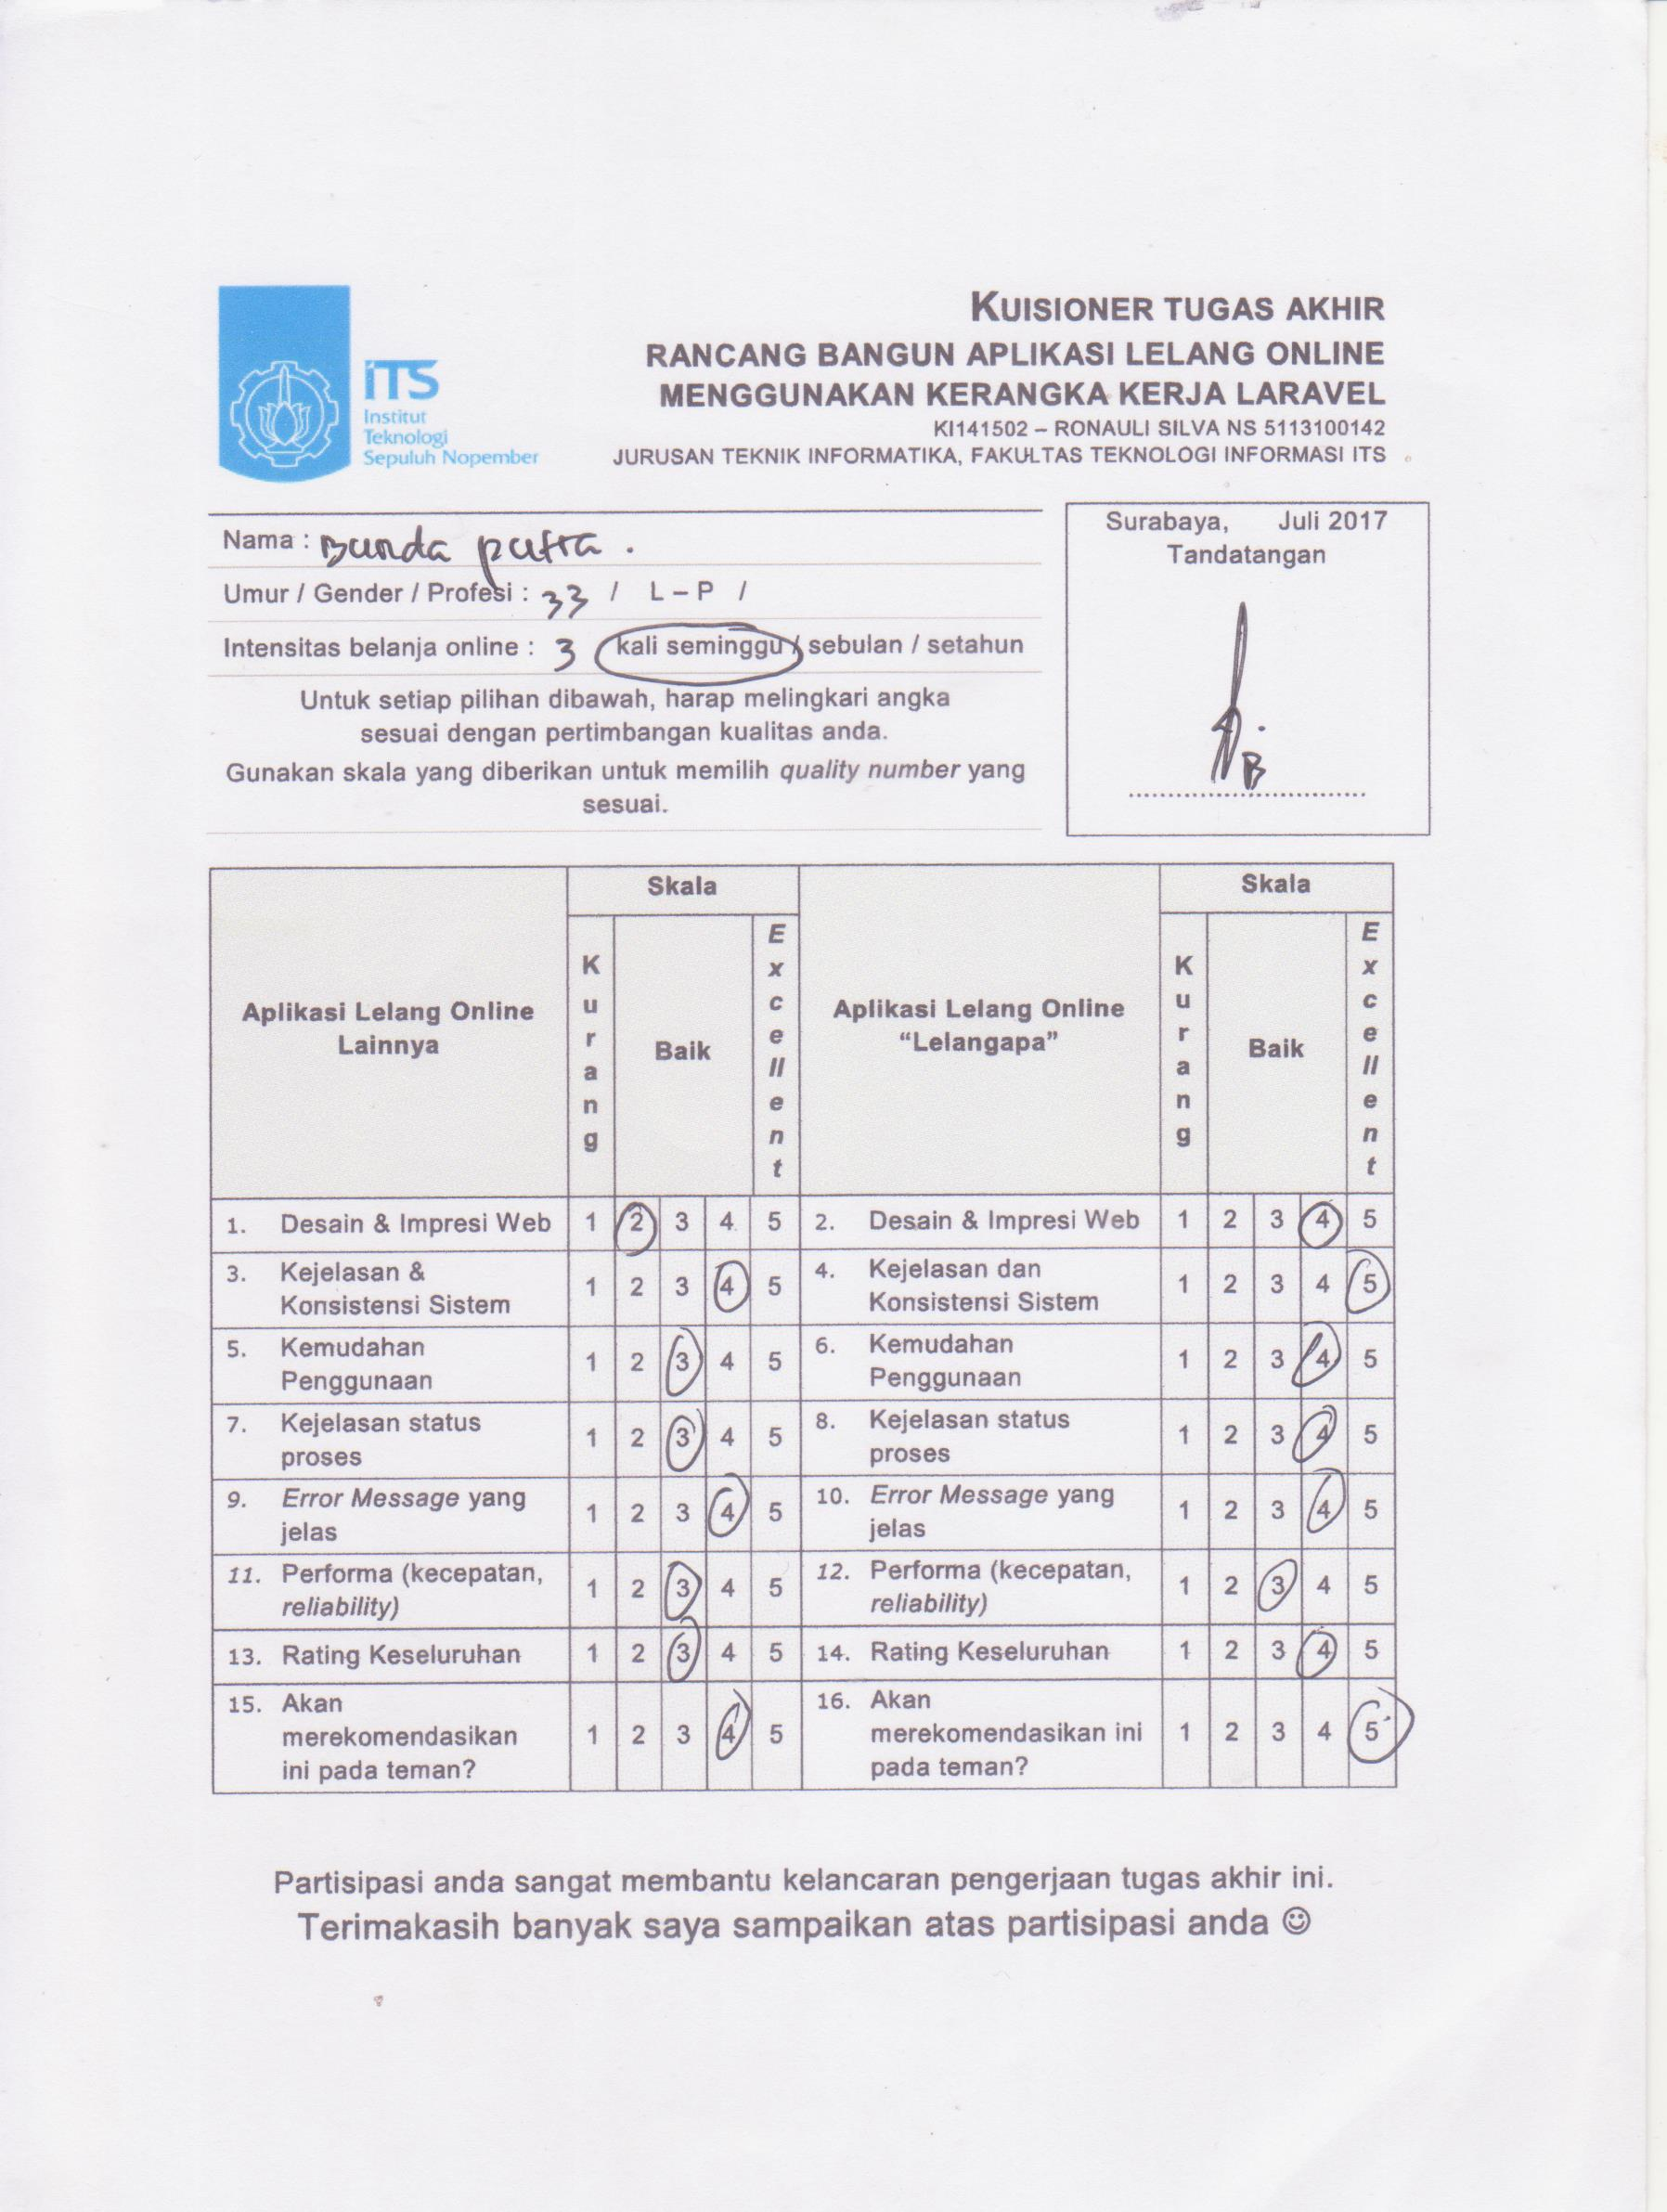
\includegraphics[width=\textwidth]{images/bab5/ujipengguna/9.jpg}
	\caption{Kuisioner Pengguna 9}
\end{figure}
\begin{figure}[H]
	\centering
	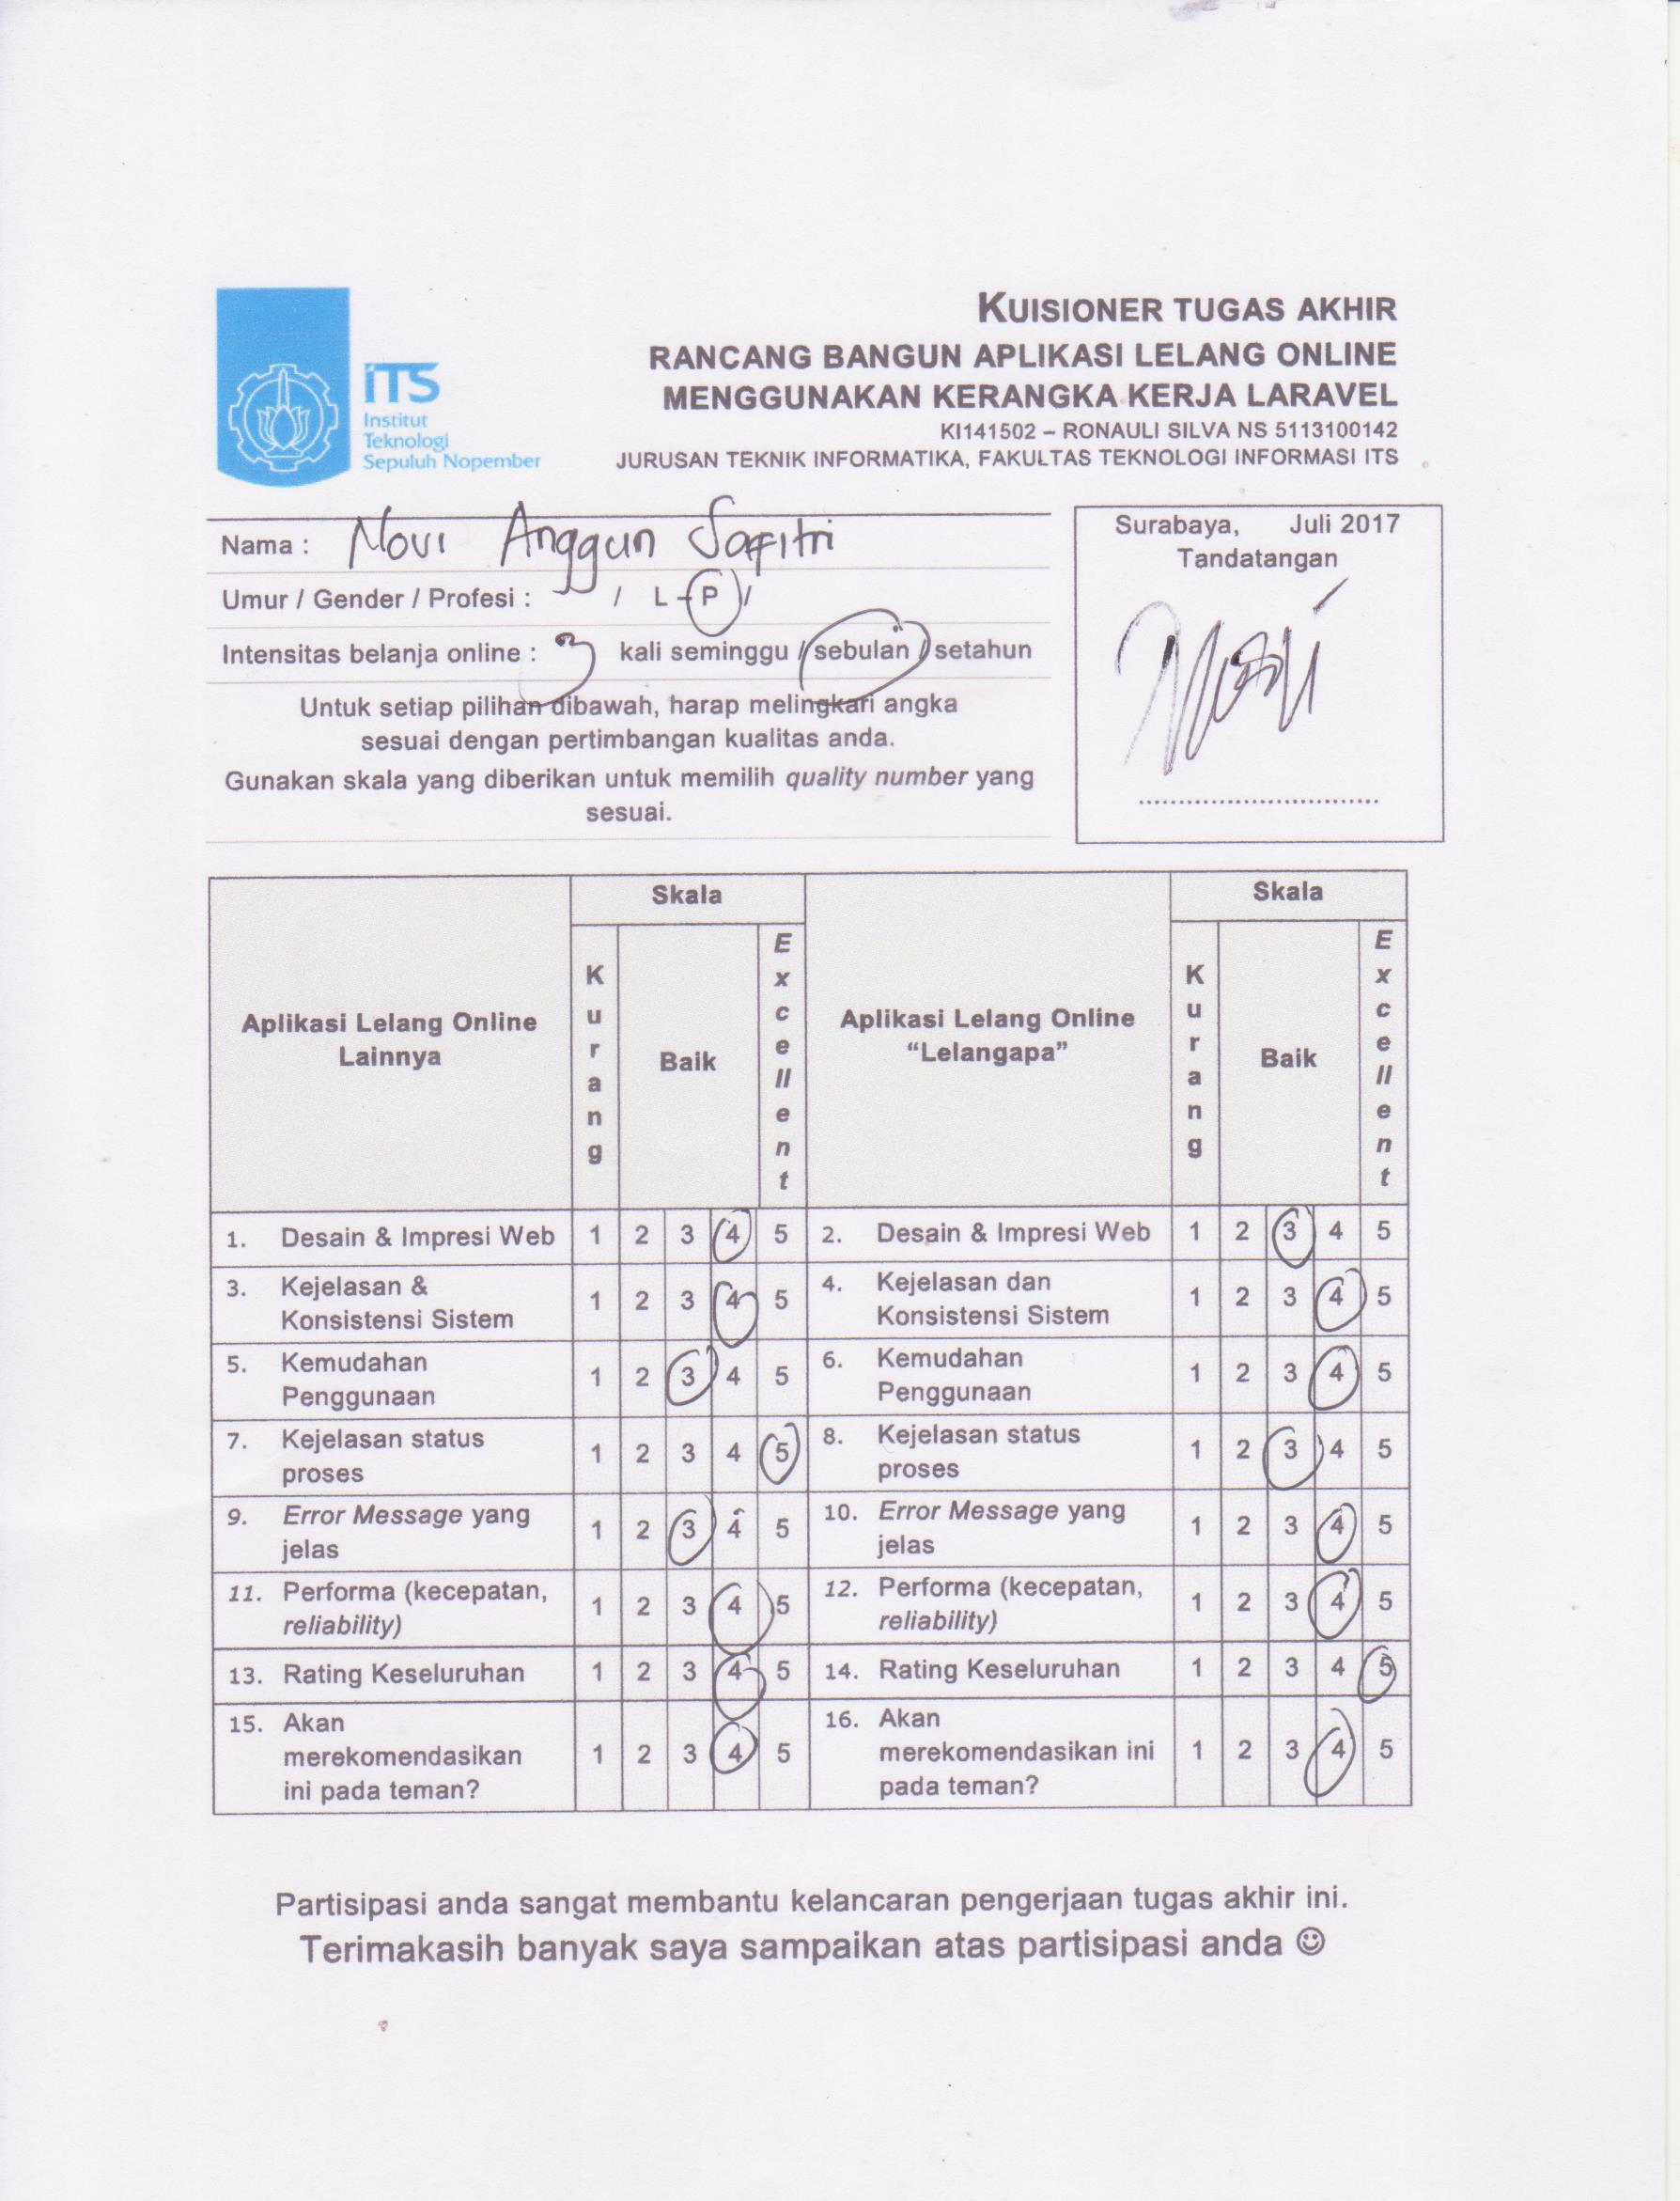
\includegraphics[width=\textwidth]{images/bab5/ujipengguna/10.jpg}
	\caption{Kuisioner Pengguna 10}
\end{figure}
\begin{figure}[H]
	\centering
	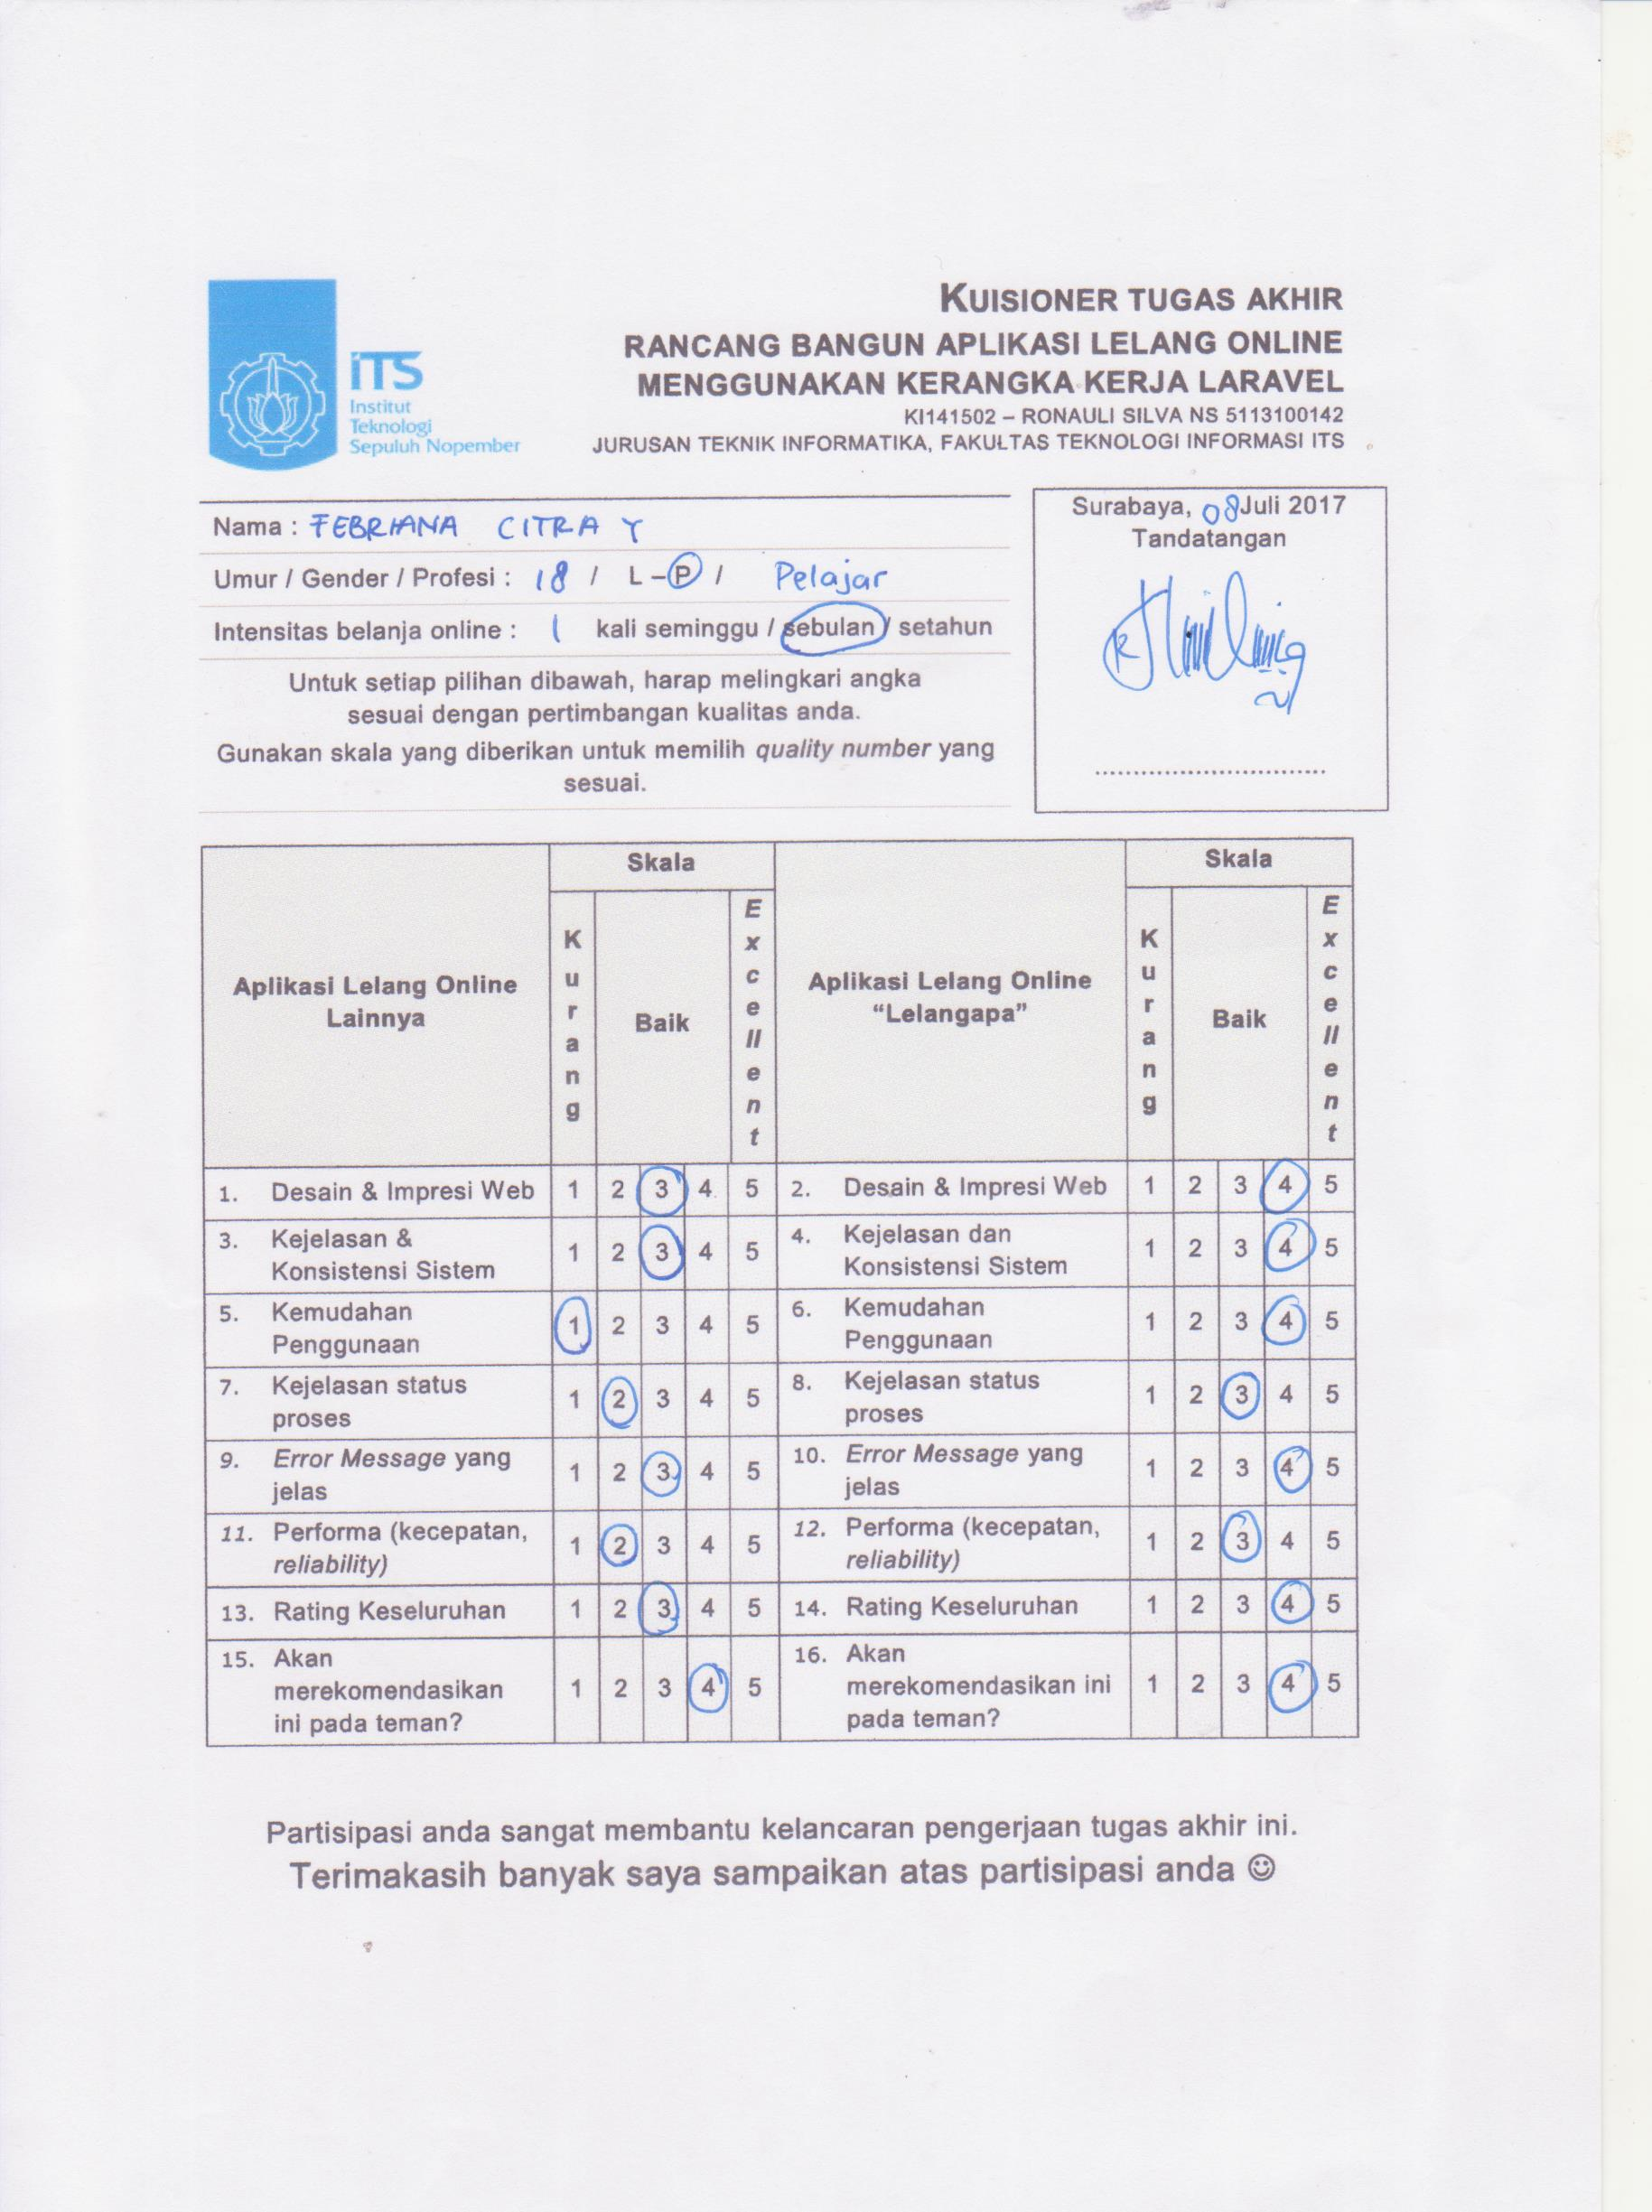
\includegraphics[width=\textwidth]{images/bab5/ujipengguna/11.jpg}
	\caption{Kuisioner Pengguna 11}
\end{figure}